\documentclass[10pt]{article}

\usepackage[a4paper,left=2cm,top=2.5cm,right=2cm,bottom=2.5cm]{geometry}
\usepackage[fleqn]{amsmath}
\usepackage{amssymb}
\usepackage{amssymb}
\usepackage{graphicx,color}
\usepackage{enumitem}
\usepackage{theorem}
\usepackage{fancybox}
\usepackage{subfigure,wrapfig}
\usepackage{bm}
\usepackage{parskip}
\usepackage{setspace}
\usepackage{caption}
\usepackage{fancyhdr}
\usepackage[compact]{titlesec}
\usepackage{url}
\usepackage{comment}
%

\setlength{\mathindent}{15mm}
% \setlength{\leftmargini}{0pt}
\setlength{\parindent}{0pt}
\setstretch{1.1}
\captionsetup{font={small,it},labelfont={bf,it}} 
\titlespacing{\section}{0pt}{*0.5}{*1}
\titlespacing{\subsection}{0pt}{*0.5}{*0.25}
\titleformat{\subsubsection}[runin]{\normalfont \bfseries \itshape}{}{0pt}{} 
\titlespacing{\section}{\parindent}{*2}{\wordsep}
\setlength{\headheight}{14pt}
\pagestyle{fancyplain}
\pagenumbering{roman}

\usepackage{fontspec}  %% xelatex or luaLatex required
\defaultfontfeatures{Scale=MatchLowercase,Mapping=tex-text}
\setmainfont{Cambria}
\setsansfont{Helvetica}
\setmonofont{Courier New}


\begin{document}


\newcommand{\dGamma}{\mathbf{d}\boldsymbol{\Gamma}}
\newcommand{\erfc}{\mbox{\rm erfc}}
\newcommand{\Red     }[1]{\textcolor[rgb]{0.7,0.0,0.0}{#1}} 
\newcommand{\Green   }[1]{\textcolor[rgb]{0.0,0.7,0.0}{ #1}} 
\newcommand{\Blue    }[1]{\textcolor[rgb]{0.0,0.0,0.7}{ #1}} 
\newcommand{\Emerald }[1]{\textcolor[rgb]{0.0,0.7,0.3}{ #1}} 


\thispagestyle{empty}
%\setlength{\unitlength}{\linewidth}


\mbox{}
\vfill

{\Large VIEPS Geodynamics --- 2015} \\[2ex]
\vfill

%\begin{figure*}[htbp]
\begin{center}
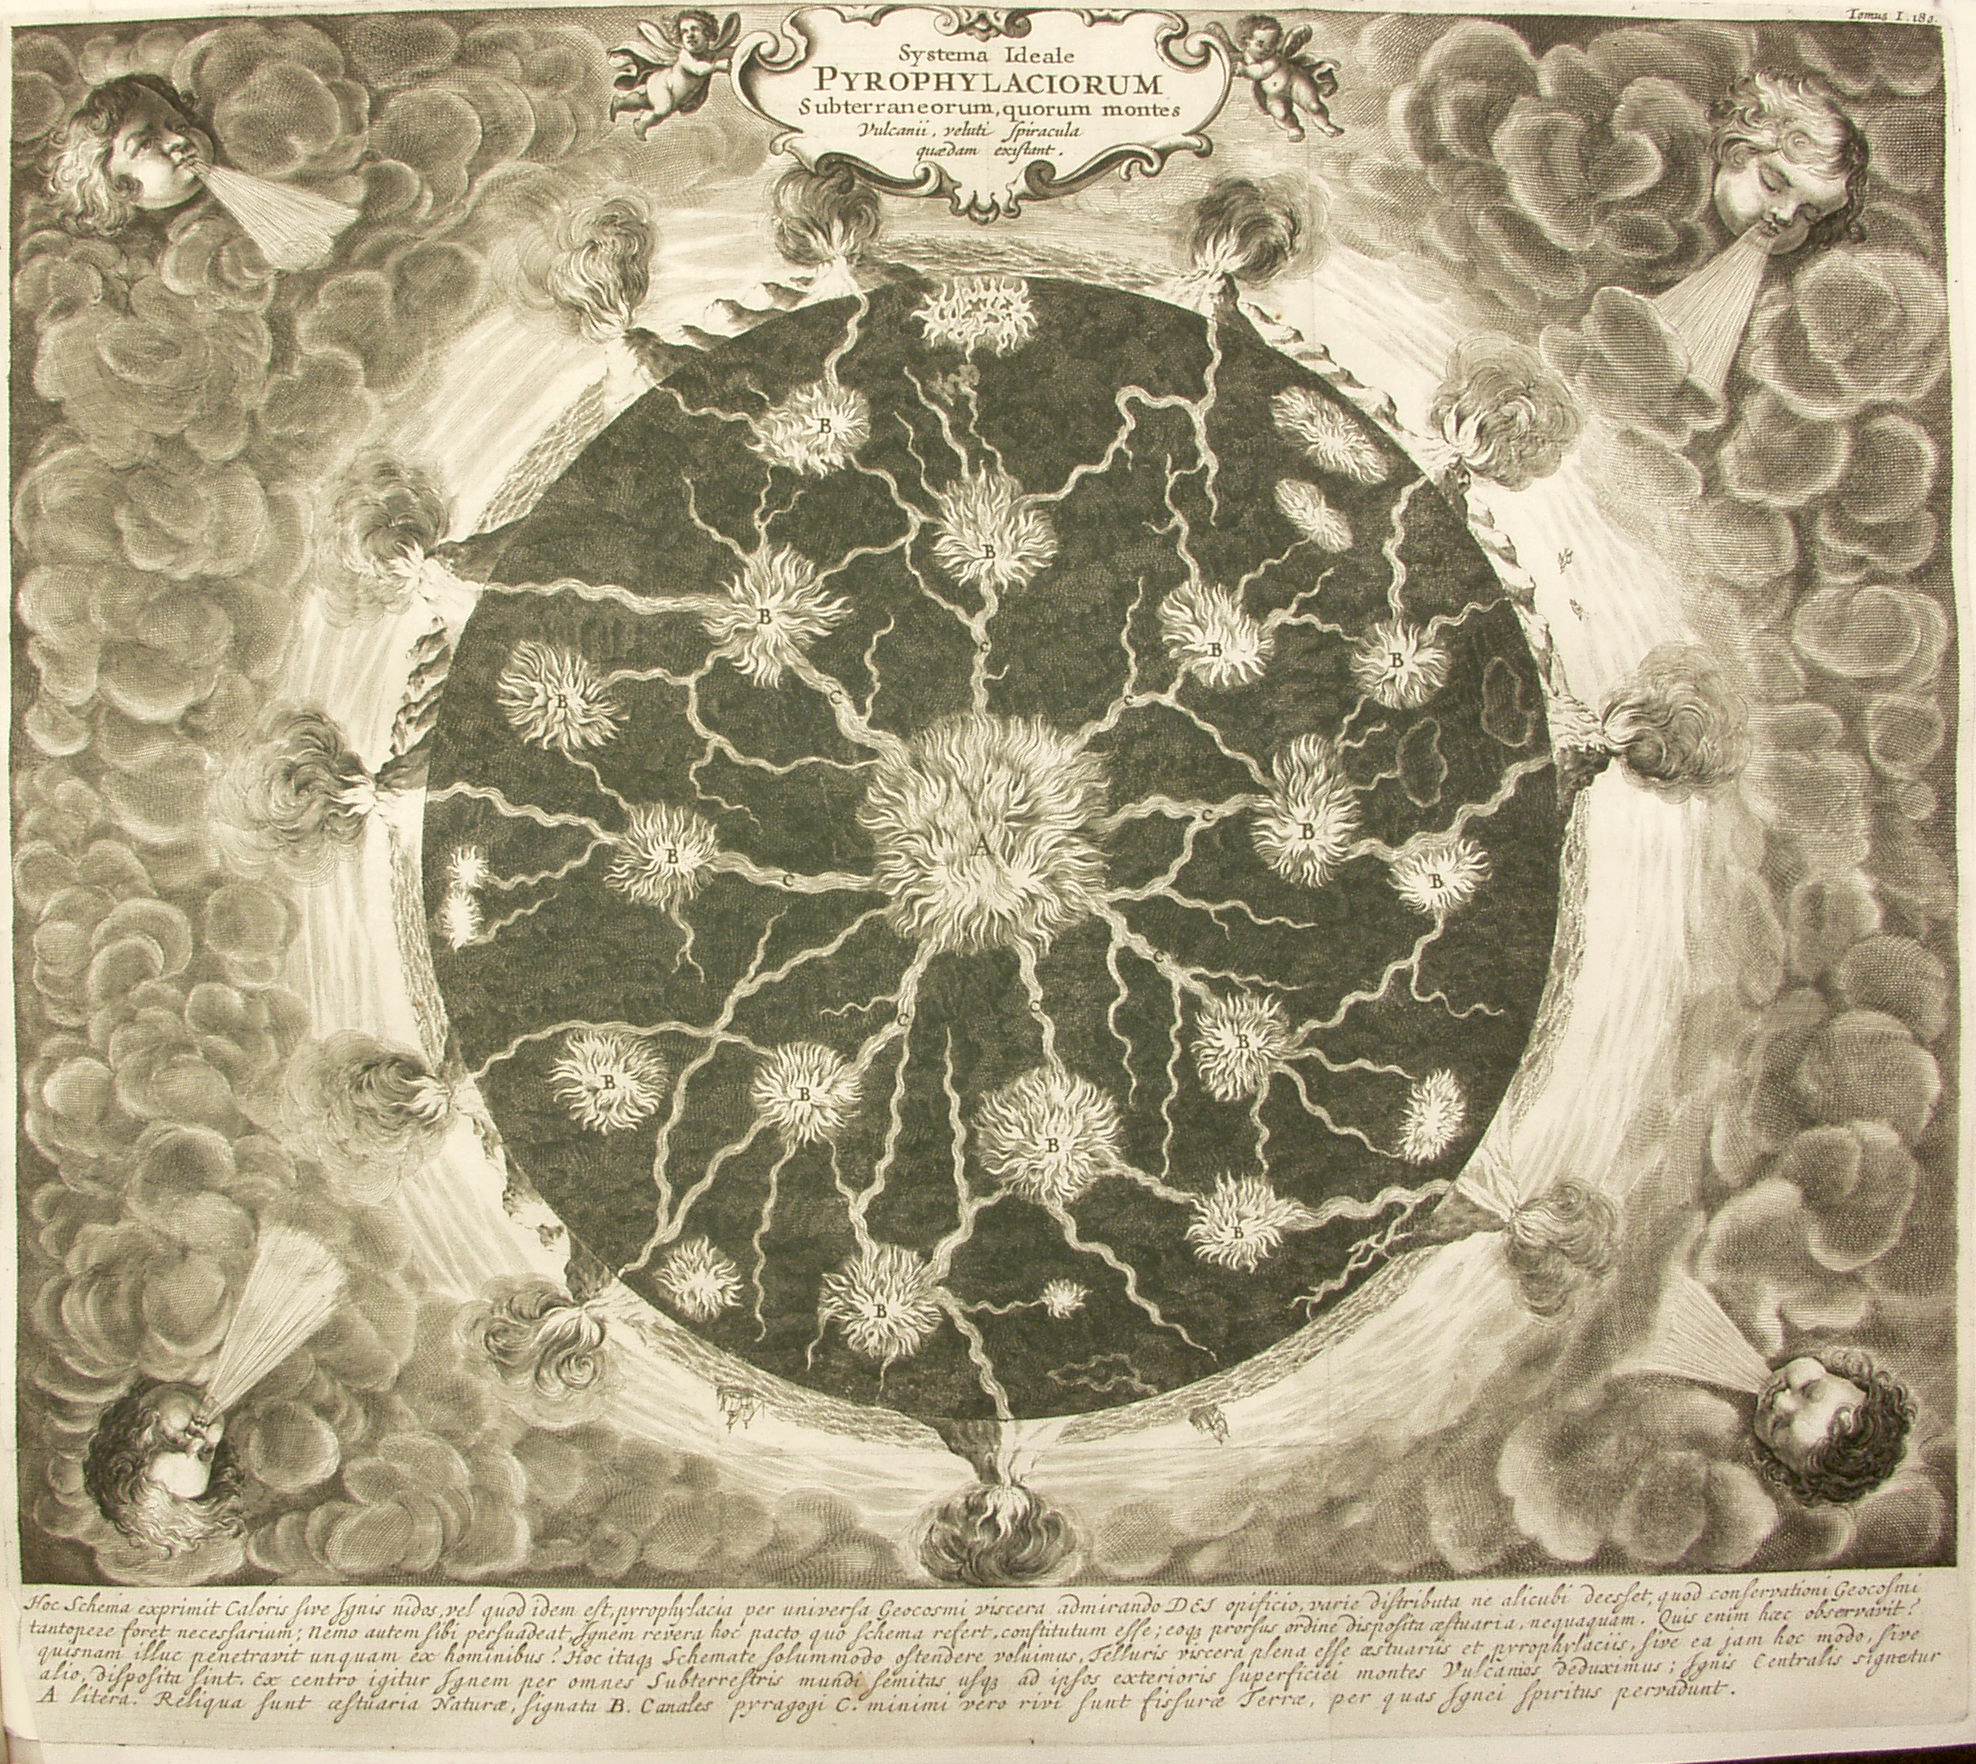
\includegraphics[width=0.9\linewidth]{MundusSubterraneusOriginal.jpg} \\[6ex]

Athanasius Kircher, Mundus subterraneus (1664/65): ``Systema Ideale PYRO-
PHYLACIORUM Subterraneorum, quorum montes \textit{Vulcanii, veluti spiracula
quaedam existant}''

\end{center}
%\end{figure*}
\vfill
{\Large Louis Moresi (louis.moresi@unimelb.edu.au)}
\vfill

\newpage


\section{Introduction} % (fold)
\label{sec:introduction}

Our goal is to develop an quantitative understanding of the dynamic processes within
the Earth and sister planets as I have sketched in the Figure to the right. These dynamic
processes are largely driven by the internal heat of the planet escaping to the surface 
through whatever mechanisms are available. Some of the heat is left over from the
original formation of the planet, and the rest originates in the decay of
radioactive elements. In the Earth's early history and elsewhere in the solar system, 
tidal heating, chemical segregation, and impacts have all played a role in supplying the 
interior heat budget. Figure \ref{fig:Diagrams_EarthProcessesPlume} is a schematic of the Earth's 
interior and something similar for Venus and Mars would be, on the face of it, much simpler.

\begin{wrapfigure}{r}{90mm} 
	\begin{center}
		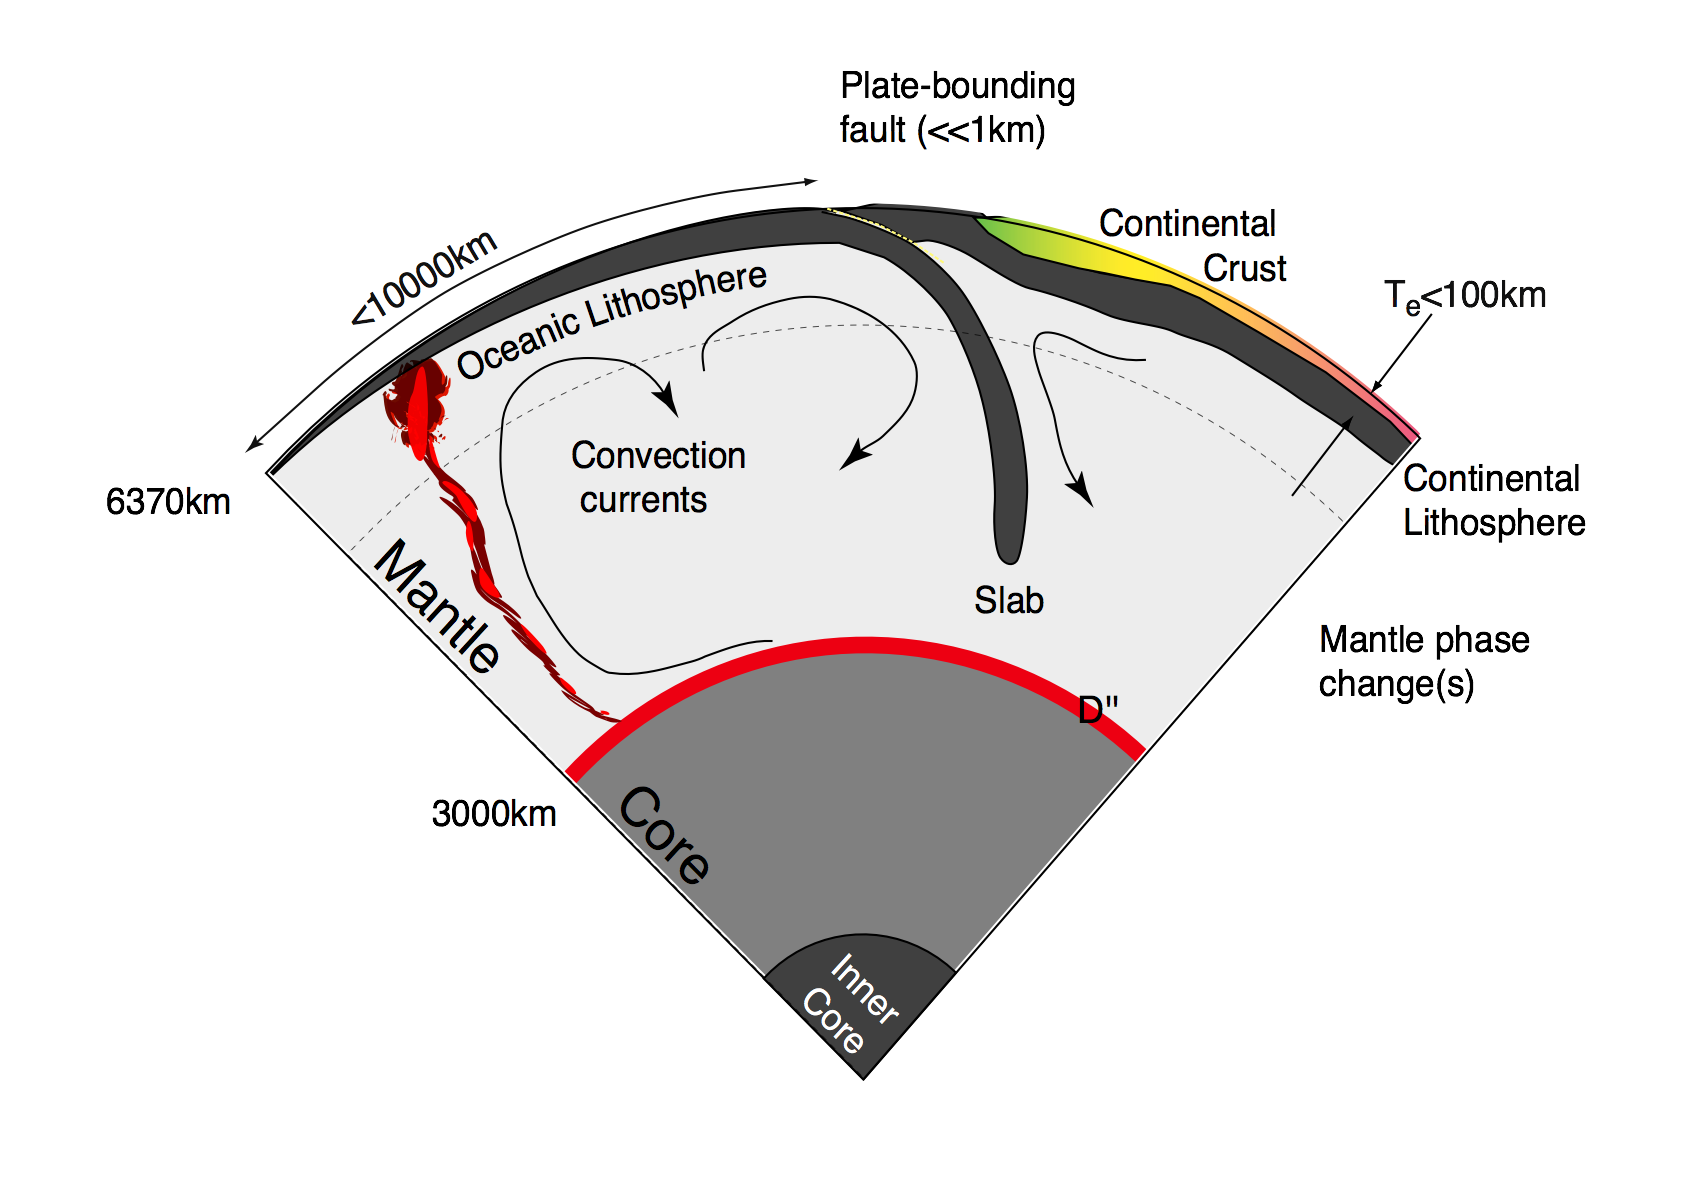
\includegraphics[width=100mm]{Diagrams/EarthProcessesPlume.png}
		 \caption[]{A schematic of the interior of the Earth showing the global 
		            scale processes we seek to understand quantitatively in this course}
	\end{center}
	\label{fig:Diagrams_EarthProcessesPlume}	
\end{wrapfigure}

This is because the Earth's dynamics is completely dominated by Plate Tectonics --- a unique
manifestation of interior heat loss as far as we are aware. Part of our task is to understand
why plate tectonics is a possible outcome of a hot planet, but also why it is not the only 
possible outcome. If we can also understand how the different modes are selected for planets
of different size, composition, and heat budget, then we have a powerful way to predict the
geological behaviour of extrasolar planets. Plate tectonics creates a number of very efficient
cycling mechanisms which link the interior of the Earth and the Atmosphere and Oceans; it may
prove to be an essential ingredient for the kind of friendly world we expect to be needed to 
nurture (intelligent) life. 

% section introduction (end)

\subsection{Modeling}

Global scale geodynamics is a discipline where we cannot
do controlled experiments on the basic processes we are studying.
We rely on observing the Earth and the other terrestrial planets and moons and
looking for multiple manifestations of the same processes under different 
conditions to give us control on certain parameters. 

While it is not possible to do experiments at the planetary scale over geological time, it is 
possible to perform experiments at a physically manageable size and, by careful
scaling, to generalise the results to geologically relevant space and time-scales. 
If these processes of interest can be understood through a mathematical description, then
the equations are automatically applicable at geological time and space scales provided the 
assumptions which go into developing the mathematical model are still valid. 

We will frequently be talking about ``modeling'' --- people mean many different 
things by this and all of the following fall under the general concept of modeling:

\begin{itemize}
	\item Laboratory based physical models which can be scaled to 
		  give meaningful, quantitative insight into deformation at geological scales.
	\item The building of mathematical descriptions of the world
	      and their use to approximate physical "reality".
	\item Computational solution of these descriptions (where needed) and
	      the concept of a numerical model.
	\item How to go about constructing a model 
	\item How to go about using a model (these are quite different things !). 
	\item Exploring parameter variation to understand the dominant effects.
\end{itemize}

%% Thunderbirds are go !! 

\subsection{Mathematical background}

These notes contains material at different levels. There is broadly descriptive
content which is intended to introduce the subject and lead up to the more advanced
mathematical content. It should be possible to follow these notes without 
detailed knowledge of how the mathematical results are obtained, but it is 
expected that you can use the results in exercises for to solve real problems
in geophysics.

Familiarity with vector \& tensor notation \& index notation is required for
understanding the kinds of equations we will be dealing with and I interchange
them a little. On the assumption that these things are disconcerting (at best)
the first few times, I tend to write everything out in full -- at least for
the Cartesian case. In other geometries, vector notation generally still
holds, but the definition of the operators can be very different, and it is
always worth checking before using them. 

\newpage
\section{Conceptual model for mantle/lithosphere dynamics}
%% FIGURE: fluid volume element and terminology.
\begin{wrapfigure}{r}{50mm} 
	\begin{center}
		 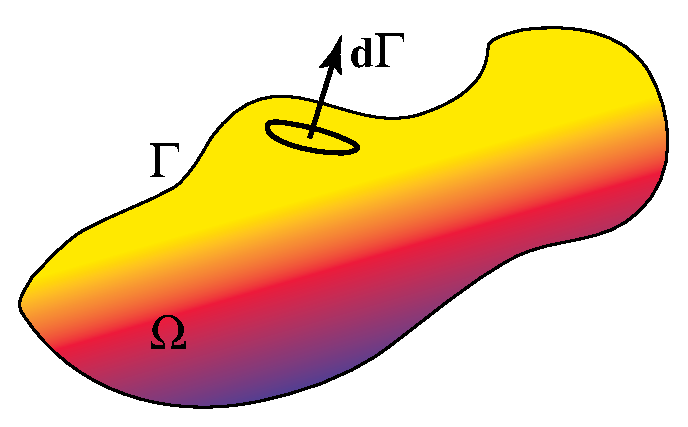
\includegraphics[width=45mm]{Diagrams/vol_elt}
		 \caption[]{Arbitrary fluid volume, $\Omega$, with surface $\Gamma$
         and elemental surface normal vector, $\dGamma$, within which the
         fluid properties are to be conserved}
	\end{center}	
\end{wrapfigure}

We start by deriving the equations of motion, energy balance and so on through
a conservation principle. This will give a useful insight into the different
forms of the equations which we will later encounter.

A general conservation law does not distinguish the quantity which is being
conserved -- it is a mathematical identity. Consider a quantity $\phi$ / unit
mass which is carried around by a fluid. We can draw an arbitrary volume,
$\Omega$ to contain some amount of this fluid at a given time. We label the
surface of the volume $\Omega$ as $\Gamma$, and define an outward surface
normal vector $\dGamma$ which is normal to the tangent plane of an
infinitesimal element of the surface and has a magnitude equal to the area of
this element.

We also define a source/sink term, $H$ / unit mass which generates/consumes
the quantity $\phi$, and a flux term, $\mathbf{F}$ which occurs across the
surface when the fluid is stationary (e.g. this might represent diffusion of
$\phi$). The rate of change of $\phi$ is given by combining the contribution
due to the source term, the stationary flux term, and the effect of motion of
the fluid.		

	\begin{equation}
		\frac{d}{dt} \int_{\Omega} \rho \phi d\Omega =
			- \int_{\Gamma} \mathbf{F} \cdot \dGamma 
			+ \int_{\Omega} \rho H d\Omega
			- \int _{\Gamma} \rho \phi \mathbf{v} \cdot \dGamma 
		\label{eq:cons1}	
	\end{equation}
		
where the final term is the change due to the fluid carrying $\phi$ through
the volume. Fluxes are positive outward (by our definition of $\dGamma$), so a
positive flux reduces $\phi$ within $d\Omega$ and negative signs are needed
for these terms.
	
	We can generally use Gauss' theorem to write surface integrals as volume integrals:
	
		\begin{equation}
				\int_{\Gamma} \phi \mathbf{u} \cdot \dGamma = \int_{\Omega}  \nabla \cdot (\phi \mathbf{u}) d\Omega
		\end{equation}
	
The test surface, $\Gamma$, and volume, $\Omega$ are assumed to be \emph{fixed
in the lab reference frame} so that the order of integration and
differentiation can be interchanged

\begin{equation}
			\frac{d}{dt} \int_\Omega \rho \phi d\Omega =
			 	\int_\Omega \frac{\partial \rho \phi}{\partial t} d\Omega
\end{equation}
	
Allowing us to write
	\begin{equation}
		\int_{\Gamma} \mathbf{F} \cdot \dGamma + 
		\int _{\Gamma} \rho \phi \mathbf{v} \cdot \dGamma =
		\int_{\Omega} \nabla \cdot (\mathbf{F} + 
		\rho \phi \mathbf{v}) d\Omega	
	\end{equation}
		
so that we rewrite the general conservation equation (\ref{eq:cons1}) as 	
	\begin{equation}
		\int_{\Omega} \left[ \frac{d \rho \phi}{dt} + 
			\nabla \cdot (\mathbf{F} + \rho \phi \mathbf{v}) 
			-\rho H \right]	d\Omega	=0
	\end{equation}
		
We can now appeal to the fact that this conservation law
holds regardless of our particular choice of volume $\Omega$ and, therefore,
the integral above can only be zero for arbitrary $\Omega$ if the enclosed
term is zero everywhere, i.e.	
	\begin{equation}
		\frac{d \rho \phi}{dt} + 
			\nabla \cdot (\mathbf{F} + \rho \phi \mathbf{v}) 
			-\rho H =0
			\label{eq:cons2}
	\end{equation}
		
	This is the general conservation rule for any property $\phi$ of a moving
fluid. We now consider several quantities and develop specific conservation
laws.	
		
\subsection{Conservation of mass}
	
In this case $\phi=1$ (since $\int_\Omega \rho d\Omega \rightarrow \mbox{mass}$), $\mathbf{F} = H = 0$.
	Thus, equation (\ref{eq:cons2}) gives	
		\begin{equation}
			\Red{\frac{\partial \rho}{\partial t} + 
				\nabla \cdot \rho \mathbf{v} = 0}
			\label{eq:masscons}
		\end{equation}
		
\subsection{Conservation of (heat) energy}
	
	The thermal energy / unit mass is $C_p T$ and the conductive heat flux
$\mathbf{F}$ is given by $ \mathbf{F} = -k \nabla T$, where $k$ is the thermal
conductivity. Then the general conservation law of (\ref{eq:cons2}) reduces to
	\begin{equation}
		\frac{\partial (\rho C_p T)}{\partial t} +
			 \nabla \cdot \left(-k \nabla T + 
			 \rho C_p T \mathbf{v}\right) - \rho H = 0
	\end{equation}
		
Rearranging with some foresight gives this
		\begin{equation}	
			\frac{C_p T}{\rho} \left[ \frac{\partial \rho}{\partial t} + 
			\nabla \cdot \rho \mathbf{v} \right] + 
			\frac{\partial C_p T}{\partial t} + 
			\mathbf{v} \cdot \nabla C_p T = 
			\frac{1}{\rho} \nabla \cdot k \nabla T + H
		\end{equation}
	
Where the term in square brackets is simply the statement of mass conservation
which vanishes identically. The constant density assumption is just to simplify the discussion at this point and will have to be
revisited later in the context of thermal convection where density changes
drive the flow.
	
	If the heat capacity, $C_p$ and thermal conductivity, $k$ are
	constants, then the conservation equation becomes
			\begin{equation}
				\Red{ \left( \frac{\partial T}{\partial t} + \mathbf{v} \cdot \nabla T \right)=
						\kappa \nabla^2 T + \frac{H}{C_p} }
				\label{eq:energycons}		
		\end{equation}
					
	where $\kappa$ is the thermal diffusivity, $\kappa = k/\rho C_p$. 
	
This equation is linear provided that the velocity field is specified and is
independent of $T$. Clearly this is generally not true.
	A new bit of notation has been defined in the process of this derivation. The meaning of
	the $\mathbf{v} \cdot \nabla$ operator is
		\begin{equation}
			\mathbf{v} \cdot \nabla \equiv v_j \frac{\partial}{\partial x_j}
		\end{equation}
	
	 For later reference, this is how it looks:
		\begin{equation}
				(\mathbf{v} \cdot \nabla) T = v_1 \frac{\partial T}{\partial x_1} + 
				v_2 \frac{\partial T}{\partial x_2} + v_3 \frac{\partial T}{\partial x_3}
		\end{equation}
		
	The Laplacian, $\nabla^2$, is this expression (for scalar $T$)
		\begin{equation}
			\nabla^2 T \equiv \frac{\partial^2 T}{\partial x_1^2} + \frac{\partial^2 T}{\partial x_2^2} + \frac{\partial^2 T}{\partial x_3^2} 
		\end{equation}	
	
	\subsection{Conservation of momentum}
	
	Momentum is a vector quantity, so the form of (\ref{eq:cons1}) is slightly different. The 
	source term in a momentum equation represents a force, and the surface flux term
	represents a stress.
		\begin{equation}
			\frac{d}{dt}\int_{\Omega} \rho \mathbf{v} d\Omega = 
			-	\int_{\Omega} \rho g \hat{\mathbf{z}} d\Omega  
			+	\int_{\Gamma} \boldsymbol{\sigma} \cdot \dGamma -
				\int_{\Gamma} \rho \mathbf{v} (\mathbf{v} \cdot \dGamma)	
				\label{eq:momcons1}
		\end{equation}
		
	Gravity acts as a body force in the vertical direction, $\hat{\mathbf{z}}$.
	We have introduced the stress tensor, $\boldsymbol{\sigma}$; the force / unit area exerted
	on an arbitrarily oriented surface with normal $\hat{\mathbf {n}}$ is 
		\begin{equation}
			f_i = \sigma_{ij} n_j
		\end{equation}	
			
	The application of Gauss' theorem, and using the arbitrary nature of 
	the chosen volume to require the integrand to be zero, as before,  gives	
		\begin{equation}
			 \frac{\partial}{\partial t}(\rho \mathbf{v}) 
			+\rho g \hat{\mathbf{z}} - \nabla \cdot \sigma + \nabla \cdot (\rho \mathbf{v} \mathbf{v}) = 0
			\label{eq:momcons2}
		\end{equation}	
		
	Vector notation allows us to keep a number of equations
	written as one single equation. However, 
	at this point, keeping the equations in vector notation
	makes the situation more confusing. Particularly, the last term
	of equation (\ref{eq:momcons2}) stretches the current notation
	rather too much. Instead, we consider the individual components of
	momentum, each of which must satisfy the conservation law 
	independently
	
	In index notation, equation (\ref{eq:momcons2}) is written as
		\begin{equation}
			\Green{\frac{\partial \rho v_i}{\partial t}} + \rho g \delta_{i3} - 
			\frac{\partial \sigma_{ij}}{\partial x_j} +
			\Blue{\frac{\partial(\rho v_i v_j)}{\partial x_j}} = 0
			\label{eq:momindx}
		\end{equation}
		
	where the troublesome final term is now  
	unambiguous. Repeated indeces in each term are
	implicitly to be summed.	$\delta_{ij}$ is the kronecker delta which obeys:
		\begin{equation}
			\delta_{ij} = \begin{cases}
				0 & \text{if $i \neq j$}, \\
				1 & \text{if $i = j$}.
			\end{cases}	
		\end{equation}
		
	With some foresight, we expand the derivatives of  products of two terms and gather up
	some of the resulting terms:
		\begin{equation}
			v_i \left[\Green{\frac{\partial \rho}{\partial t}} +
			 \Blue{ \frac{\partial \rho v_j}{\partial x_j}} \right]
			+ \Green{\rho \frac{\partial v_i}{\partial t}} + \Blue{\rho v_j \frac{\partial v_i}{\partial x_j}} =
			\frac{\partial \sigma_{ij}}{\partial x_j} -\rho g \delta_{i3} 
		\end{equation}
	
	The term in square brackets is, in fact, a restatement of the conservation of mass derived above and 
	must vanish. The remaining terms can now be written out in vector notation as
		\begin{equation}
			\Red{	\rho \left( \frac{\partial \mathbf{v}}{\partial t}
							+ (\mathbf{v} \cdot \nabla) \mathbf{v} \right) =
						 \nabla \cdot \boldsymbol{\sigma} - g\rho\hat{\mathbf{z}}      }
			\label{eq:momcons3}
		\end{equation}

	Note: The $\mathbf{v} \cdot \nabla$ notation we introduced earlier is 
	now an operator on a vector. In this context, the $\mathbf{v} \cdot \nabla$ 
	operator acts on each component of the vector independently. Written out
	it looks like this:
	 		\begin{equation}
	 			\begin{split}
					(\mathbf{v} \cdot \nabla) \mathbf{u} = 
						& \hat{\boldsymbol{\imath}} \left( v_1 \frac{\partial u_1}{\partial x_1} + 
						v_2 \frac{\partial u_1}{\partial x_2} + v_3 \frac{\partial u_1}{\partial x_3} \right) \\
							& \hat{\boldsymbol{\jmath}} \left( v_1 \frac{\partial u_2}{\partial x_1} + 
						v_2 \frac{\partial u_2}{\partial x_2} + v_3 \frac{\partial u_2}{\partial x_3} \right) \\
							& \hat{\boldsymbol{k}} \left( v_1 \frac{\partial u_3}{\partial x_1} + 
						v_2 \frac{\partial u_3}{\partial x_2} + v_3 \frac{\partial u_3}{\partial x_3} \right) \\				
				\end{split}	
		\end{equation}
	 

\section{Constitutive Laws}
	
	The formulation above is quite general, and can be extended where necessary to include 
	conservation laws for additional physical variables (for example, angular momentum, electric current).
	Specific to the type of material which is deforming is the constitutive law which 
	describes the stress. In the case of an incompressible fluid, the stress is related to strain rate through
	a viscosity, $\eta$, and to the pressure, $p$. Incompressibility
	is expressed as	
		\begin{equation}
			\nabla \cdot \mathbf{u} = 0	
		\end{equation}
	
	This is a tighter constraint than mass conservation and emerges from 
	equation (\ref{eq:masscons}) when $\rho$ is 
	assumed to be constant. With this assumption, the constitutive law is written
	\Emerald{(A derivation for this is in Landau \& Lifschitz). }
		\begin{equation}
			\sigma_{ij} = \eta \left( \frac{\partial v_i}{\partial x_j} + \frac{\partial v_j}{\partial x_i}\right) - p\delta_{ij}
		\end{equation}
	
	If the viscosity is constant, then we can substitute the constitutive law 
	into the stress-divergence term of the momentum conservation equation.
	In index notation once again,
		\begin{equation}
			\begin{split}
				\nabla \cdot \boldsymbol{\sigma} & =
					\frac{\partial}{\partial x_j} \eta 
						\left( \frac{\partial v_i}{\partial x_j} +	\frac{\partial v_j}{\partial x_i} \right)
						- \frac{\partial p}{\partial x_j} \delta_{ij} \\
				& = \eta \frac{\partial^2 v_i}{\partial x_j \partial x_j} +
							\eta \frac{\partial^2 v_j}{\partial x_i \partial x_j} -
								\frac{\partial p}{\partial x_i}\\
				& = \eta \nabla^2 \mathbf{v} +
				             \eta \Green{\nabla (\nabla \cdot \mathbf{v})} - \nabla p 		
			\end{split}		
		\end{equation}
	
	the second term in this final form must vanish because of 
	the incompressibility assumption, so the momentum conservation equation becomes
		
			\begin{equation}
				\Red{	\rho \left( \frac{\partial \mathbf{v}}{\partial t}
							+ (\mathbf{v} \cdot \nabla) \mathbf{v} \right) =
						 	\eta \nabla^2 \mathbf{v} - \nabla p	
						 	- g\rho\hat{\mathbf{z}}      }
				\label{eq:navstokes}		 	
			\end{equation}
	
	This is the Navier-Stokes equation.
	Once again some new notation has shown up uninvited. The Laplacian
	operator $\nabla^2$ is defined (in a scalar context) as
		\begin{equation}
			\begin{split}
			\nabla^2 \phi & = \nabla \cdot \nabla \phi \\
									& =	\frac{\partial^2 \phi}{\partial x^2} + 
											\frac{\partial^2 \phi}{\partial y^2} + 	
											\frac{\partial^2 \phi}{\partial z^2}  \text{\hspace{1cm} (Cartesian)}
			\end{split}
		\end{equation}
	
	and in a vector context as
		\begin{equation}
			\begin{split}
				\nabla^2 \mathbf{u} & = \nabla \nabla \cdot \mathbf{u} - \nabla \times (\nabla \times \mathbf{u}) \\
													& =	\mathbf{i} \nabla \cdot \nabla u_x + 
															\mathbf{j} \nabla \cdot \nabla u_y + 
															\mathbf{k} \nabla \cdot \nabla u_z   \text{\hspace{1cm} (Cartesian)}
			\end{split}
		\end{equation}
	
	In Cartesian coordinates, the Laplacian operator has a simple form, and the vector Laplacian is simply
	the scalar operator applied in each direction. In other coordinate systems this operator becomes
	substantially more elaborate. 
	
%TODO  \Emerald{(Example !!)}
	
	
\section{Boussinesq Approximation, Equation of State, Density Variations}
	
	The equation which relates pressure, temperature and 
	density is known as the equation of state. For the equations
	derived so far, we have specified an incompressible fluid, for which 
	no density variations are possible. However, we have also 
	included a source term for momentum which relies on gravity
	acting on {\em density variations}.
	
	This conflict is typical of fluid mechanics: simplifying assumptions
	if taken to their logical limit imply no motion or some other trivial
	solution to the equations. 
	
	In this case, we make the assumption that density changes are typically
	small relative to the overall magnitude of the density itself. Terms which
	are scaled by density can therefore assume that it is a large constant value. 
	Terms which contain gradients of density or density variations should consider
	the equation of state. This is the Boussinesq approximation and is only a suitable
	appropriation for nearly- incompressible fluids. In the Navier-Stokes equation,
	the hydrostatic pressure does not influence the velocity field at all. 
	Only \textit{differences} in density drive fluid flow, and so the sole term in which
	density needs to be considered variable is that of the gravitational body forces.
	
	In the case of density variations due to temperature, the equation of state
	is simply
		\begin{equation}
			\rho = \rho_0 \left(1 - \alpha ( T-T_0 )\right)
			\label{eq:state}
		\end{equation}
		
	where $\rho_0$ is the density at a reference temperature $T_0$. $\alpha$ is
	the coefficient of thermal expansion. It is generally much smaller than one, making
	the Boussinesq approximation a reasonable choice.
	
	The energy and momentum
	conservation equations thus become coupled through the term
		\begin{equation}
			g\rho\hat{\mathbf{z}} = g \rho_0 \left(1 - \alpha(T-T_0)\right)
		\end{equation}
		
	Density variations due to pressure produce a perfectly vertical, isotropic
	forcing term on the momentum conservation equation. In the steady
	state case, this is balanced 
	by the hydrostatic pressure gradient. (The isotropic term does not
	contribute at all the the deviatoric part of the stress equation and thus
	cannot induce steady flow). We therefore ignore the vertical density
	gradient due to the fluid overburden.
	
	Another density variation is that which results from 
	variation in chemical composition from one fluid element to
	another. This is the case where two immiscible fluids live in
	the same region. Now density variations might be large -- the
	fluid domains must be considered separately.
	
\subsection{Advection and the Lagrangian  Formulation}
	
	We have seen the $\mathbf{v} \cdot \nabla$ operator a number of times now.
	The presence of this term causes major difficulties in continuum mechanics since
	it introduces a strong non-linearity into the momentum equation. It is this
	term which produces turbulence in high speed flows etc.
	
	This term is the `advection' term which accounts for the passive transport of
	information (temperature, momentum, by the motion of the fluid. Advection
	also presents some serious headaches in numerical methods and has spawned
	entire literatures devoted to efficient and accurate solution methods.
	
	One obvious way to avoid the problem of advection is to consider an elemental
	volume of space which {\em moves with the fluid}. The surface flux term from 
	equation (\ref{eq:cons1}) vanishes immediately
	
	Mathematically, we introduce a new notation (of course), as follows:
		\begin{equation}
			\frac{D \phi}{D t} = \frac{d}{dt} \phi[x_1(t),x_2(t),x_3(t),t]
		\end{equation}
	
 	where the change in the reference position $(x_1(t),x_2(t),x_3(t))$ is 
 	governed by the local flow velocity:
 		\begin{equation}
 					\frac{d x_1}{d t} = v_1 \mbox{\hspace{1cm}}
 					\frac{d x_2}{d t} = v_2 \mbox{\hspace{1cm}}
 					\frac{d x_3}{d t} = v_3
		\end{equation}
		
	which keeps the reference point moving with the fluid. Differentiating gives	
		\begin{align}
				\frac{D \phi}{D t} &= \frac{\partial \phi}{\partial t}
									\frac{\partial \phi}{\partial x_1}\frac{d x_1}{d t} + 
									\frac{\partial \phi}{\partial x_2}\frac{d x_2}{d t} +
									\frac{\partial \phi}{\partial x_3}\frac{d x_3}{d t} \nonumber \\
		\intertext{and so leads to}
				\frac{D \phi}{D t} &= 	\frac{\partial \phi}{\partial t}
									v_1 \frac{\partial \phi}{\partial x_1} + 
									v_2 \frac{\partial \phi}{\partial x_2} +
									v_3 \frac{\partial \phi}{\partial x_3}  \nonumber \\
		\intertext{which is equivalent to}
				\frac{D \phi}{D t} &= \frac{\partial \phi}{\partial t} + (\mathbf{v} \cdot \nabla) \phi							
		\end{align}		
					
	If we think of $\phi$ as the concentration of a dye in the fluid, then the above is
	a conservation equation assuming the dye does not diffuse and has no sources
	or sinks.				
					
	Viewed from a reference frame locked to {\em a particular fluid element}, the 
	energy conservation equation becomes
		\begin{equation}
				% \rho  ??
				\frac{D T}{Dt} =
						\kappa \nabla^2 T + \frac{H}{C_p}
		\end{equation}
		
	and the momentum conservation equation now becomes
		\begin{equation}
			\rho %% ?
			\frac{D \mathbf{v} }{D t} =
						 	\eta \nabla^2 \mathbf{v} - \nabla P 	
						 	- g\rho\hat{\mathbf{z}}      
		\end{equation}		
				
	This is a considerably more compact way of writing the equations, but  
	we have only really succeeded in hiding the nasty term under the rug, since
	it is now necessary to use a coordinate system which is locked into the fluid
	and rapidly deforms as the fluid flows. Before long, the coordinate system
	is unimaginably complex -- the advection problem returns in another guise. This
	formulation is known as the Lagrangian formulation and contrasts with
	the Eulerian viewpoint which is fixed in space.
	
	From the numerical point of view, however, this approach can have some 
	distinct advantages. The computer can often track the distorted coordinate
	system far better than it can handle successive applications of the 
	$\mathbf{v} \cdot \nabla$ operator at a fixed point in space. We
	will return to this point later.
	
	\section{Non-dimensional equations \& dimensionless numbers}
	

	%% \Emerald{Example from T. E. Faber on Dimensional Analysis}
	
	Before too long it would be a good idea to get a feeling for the 
	flavour of these equations which continual rearrangements will not
	do — it is necessary to examine some solutions. 
	
	First of all, however, it is a good idea to make some simplifications
	based on the kinds of problems we will want to attack. The first
	thing to do, as is often the case when developing a model, is to
	test whether any of the terms in the equations are negligibly
	small, or utterly dominant.  This is done by, essentially, dimensional
	analysis.
	
	Now we consider some `typical values' for the independent
	dimensions of the system (mass, length, time, temperature, that sort of thing) which
	can be used to rescale the standard units.  We rescale all lengths
	by the depth of the fluid, $d$ (e.g. mantle thickness or depth of 
	fluid in a lab tank),  time according to the characteristic time for 
	diffusion of heat, and temperature by the temperature difference 
	across the depth of the layer. Obviously these choices are 
	dependent on the problem in question but this exercise is
	a common one in fluid dynamics and provides a useful first
	step in the assault on the problem
	
	%% FIGURE: sketch of motion in a layer
		\begin{figure}[h]
			\begin{center}
				%\epsfxsize=6cm \epsfbox{:Diagrams:layer.eps}
				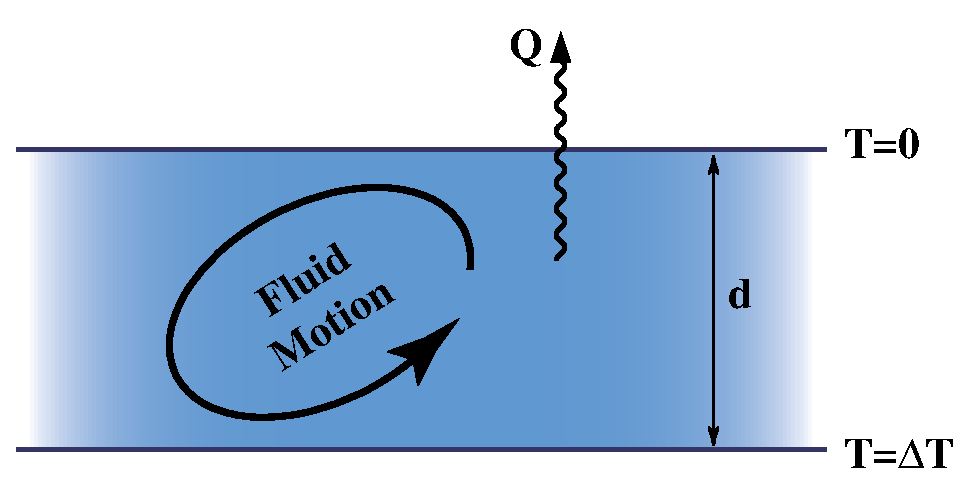
\includegraphics[width=60mm]{Diagrams/layer}				
				\caption[]{Consider the fluid motions in a layer of arbitrary depth, $d$. The fluid
				is assumed to have constant properties such as viscosity, thermal expansivity,
				thermal diffusivity. Small fluctuations in density due to temperature driven flow.
				Additional heat is carried (advected) by the flow from the hot boundary to the
				cool one whenever the fluid is moving.}
			\end{center}	
		\end{figure}
	
	Various scalings result, with the new variables indicated using a
	prime ($'$).
		\begin{equation}
			\begin{array}{llll}
				x = d.x' & \partial / \partial x = 	(1/d) \partial / \partial x' & \nabla = (1/d) \nabla '  \\
				t = (d^2/\kappa) t'  &  \partial / \partial t = (\kappa/d^2) \partial / \partial t' & \\
				T = \Delta T T' & & \\
				v = (\kappa / d) v' && \\
				p= p_0 + (\eta \kappa / d^2) p'
			\end{array}
		\end{equation}
	
	where 
		\begin{equation}
			\nabla p_0 = - g \rho_0 
		\end{equation}
	
	Substituting for all the existing terms in the Navier-Stokes equation (\ref{eq:navstokes}) 
	using the equation of state for thermally induced variation in density (\ref{eq:state}) gives:
		\begin{equation}
			\frac{\rho_0 \kappa}{d^2} \frac{D}{Dt'} \left( \frac{\kappa}{d} \mathbf{v}' \right) =
				\frac{\eta}{d^2} \acute{\nabla}^2 \left( \frac{\kappa}{d} \mathbf{v}' \right)
				- \frac{\eta \kappa}{d^3}  \acute{\nabla} p' + g \rho_0 \alpha \Delta T T' \hat{\mathbf{z}}
		\end{equation}
	
	Collecting everything together gives 
		\begin{equation}
			\frac{\rho_0 \kappa^2}{d^3} \frac{D\mathbf{v}'}{Dt'}  =
				\frac{\eta \kappa}{d^3} \acute{\nabla}^2  \mathbf{v}' 
				- \frac{\eta \kappa}{d^3}  \acute{\nabla} p' + g \rho_0 \alpha \Delta T T' \hat{\mathbf{z}}
		\end{equation}
	
	Divide throughout by $\eta \kappa / d^3$ gives
		%% \begin{equation}
			\begin{align}
				\frac{\rho \kappa}{\eta} \frac{D\mathbf{v}'}{Dt'}  & =
					 \acute{\nabla}^2  \mathbf{v}'  -  \acute{\nabla} p' + 
					 \frac{g \rho_0 \alpha \Delta T d^3}{\kappa \eta} T' \hat{\mathbf{z}} \nonumber \\
			\intertext{or}	 
				\frac{1}{{\rm Pr}} \frac{D\mathbf{v}'}{Dt'} & =
					\acute{\nabla}^2  \mathbf{v}'  -  \acute{\nabla} p' + {\rm Ra} T' \hat{\mathbf{z}}
			\end{align}
		%% \end{equation}
	
	$\rm Pr$ is known as the Prandtl number, and $\rm Ra$ is known as the Rayleigh number; both
	are non-dimensional numbers.
	By choosing to scale the equations (and this is still perfectly general as we haven't 
	forced any particular choice of scaling yet), we have condensed the different physical
	variable quantities into just two numbers. The benefit of this procedure is that
	it tells us how different quantities trade off against one another. For example, we
	see that if the density doubles, and the viscosity doubles, then the solution should
	remain unchanged.
	
	In fact, the main purpose of this particular exercise is about to be revealed. The 
	value of mantle viscosity is believed to lie somewhere between $10^{19}$ and 
	$10^{23}$ ${\rm Pa . s}$, the thermal diffusivity is around $10^{-6}{\rm m}^2{\rm s}^{-1}$,
	and density around $3300 {\rm kg . m}^{-3}$. This gives a Prandtl number greater than
	$10^{20}$. Typical estimates for the Rayleigh number are between $10^6$ and $10^8$
	depending on the supposed depth of convection, and the uncertain mantle viscosity. 
	
Obviously, the time-dependent term can be neglected for the mantle, since it
is at least twenty orders of magnitude smaller than other terms in the
equations. The benefit of this is that the nasty advection term for momentum
is eliminated -- flow in the mantle is at the opposite extreme to turbulent
flow. The disadvantage is that the equations now become non-local: changes in
the stress field are propogated instantly from point to point which can make
the equations a lot harder to solve. This can be counter-intuitive but the
consequences are important when considering the dynamic response of the Earth
to changes in, for example, plate configurations.

 Incidentally, a third, independent dimensionless number can be derived for
the thermally driven flow equations. This is the Nusselt number
\begin{equation}
			{\rm Nu} = \frac{Q}{k\Delta T}
\end{equation}
		
and is the ratio of actual heat transported by fluid motions in the layer compared to that transported conductively in the absence of fluid motion.

 All other dimensionless quantities for this system can be expressed as some
combination of the Nusselt, Rayleigh and Prandtl numbers. The Prandtl number
is a property of the fluid itself -- typical values are: air, $\sim$1; water,
$\sim$ 6; non-conducting fluids $10^3$ or more; liquid metal, $\sim$0.1.
Rayleigh number and Nusselt number are both properties of the chosen geometry.
	
	
\subsection{Stream function / Vorticity Notation}
			
For incompressible flows in two dimensions it can be very convenient to work
with the stream-function -- a scalar quantity which defines the flow
everywhere. Another quantity much beloved of fluid dynamicists is the
vorticity. Although the application of such quantities to deformation of the
solid planets is actually quite limited, it is still useful for exploring the basic fluid dynamics of the large scale flow.
			
\subsubsection{Streamfunction}
			
		The stream function is the scalar quantity,$\psi$, which satisfies
			\begin{equation}
						v_1 = -\frac{\partial \psi}{\partial x_2} \mbox{\hspace{1cm}}
						v_2 = \frac{\partial \psi}{\partial x_1}
					\label{eq:strmfn}	
			\end{equation}
		so that, automatically, 
			\begin{equation}
				\frac{\partial v_1}{\partial x_1} + \frac{\partial v_2}{\partial x_2} = 0
			\end{equation}	
			
		Importantly, computing the following
			\begin{equation}
				(\mathbf{v} \cdot \nabla) \psi = 
						v_1 \frac{\partial \psi}{\partial x_1} + 	
						v_2 \frac{\partial \psi}{\partial x_2} = 
						\frac{\partial \psi}{\partial x_2} \frac{\partial \psi}{\partial x_1} -
						\frac{\partial \psi}{\partial x_1} \frac{\partial \psi}{\partial x_2} = 0
			\end{equation}
		tells us that $\psi$ does not change due to advection -- in other words, contours
		of constant $\psi$ are streamlines of the fluid.
		
		Provided we limit ourselves to the xy plane, it is possible to 
		think of equation (\ref{eq:strmfn}) as
			\begin{equation}
					\mathbf{v} = \nabla \times (\psi \hat{\mathbf{k}})
			\end{equation}
		
			This form can be used to write down the2D axisymetric version of 
		equation  (\ref{eq:strmfn}) at once
			\begin{eqnarray}
					u_r = -\frac{1}{r}\frac{\partial \psi}{\partial \theta} & & 
					u_\theta = \frac{\partial \psi}{\partial r}
			\end{eqnarray}
		which automatically satisfies the incompressibility condition in plane
		polar coordinates
			\begin{equation}
				\frac{1}{r}\frac{\partial}{\partial r}(ru_r) + \frac{1}{r}\frac{\partial u_\theta}{\partial \theta} = 0
			\end{equation}
		
		\subsubsection{Vorticity}
		
Vorticity is defined by
	\begin{equation}
		\boldsymbol{\omega} = \nabla \times \mathbf{v}
	\end{equation}
		
In 2D, the vorticity can be regarded as a scalar as it has only one component
which lies out of the plane of the flow.

	\begin{equation}
		\omega = \frac{\partial v_2}{\partial x_1} -
		 \frac{\partial v_1}{\partial x_2}
	\end{equation}
which is also exactly equal to twice the local measure of the spin in the fluid. 
Local here means that it applies to an infinitessimal region around the sample point but
not to the fluid as a whole.

This concept is most useful in the context of invicid flow where vorticity is
conserved within the bulk of the fluid provided the fluid is subject to only conservative forces --
that is ones which can be described as the gradient of a single-valued potential.

In the context of viscous flow, the viscous effects acts cause diffusion of
vorticity, and in our context, the fact that buoyancy forces result from to
(irreversible) heat transport means that vorticity has sources. Taking the
curl of the Navier-Stokes equation, and substituting for the vorticity where
possible gives
			\begin{equation}
				\frac{1}{\rm Pr} \left( \frac{D \boldsymbol{\omega}}{D t} - 
				(\boldsymbol{\omega} \cdot \nabla) \mathbf{v} \right) = 
					\eta \nabla ^2 \boldsymbol{\omega} + {\rm Ra} \frac{\partial T}{\partial x_1}
			\end{equation}
		The pressure drops out because $\nabla \times \nabla P = 0 \mbox{\hspace{0.5cm}} \forall P$. 
		
		\subsubsection{Stream-function, Vorticity formulation}
		
		In the context of highly viscous fluids in 2D,  the vorticity equation  is
			\begin{equation}
				\nabla ^2 \omega = - Ra \frac{\partial T}{\partial x_1}
				\label{eq:vorteqn}
			\end{equation}
		and, by considering the curl of 
		$(-\partial \psi / \partial x_2, \partial \psi / \partial x_1, 0)$
		the stream function can be written
			\begin{equation}
				\nabla ^2 \psi = \omega
				\label{eq:psivort}
			\end{equation}
		
This form is useful from a computational point of view because it is
      relatively easy to solve the Laplacian, and the code can be reused for
      each application of the operator. The Laplacian is also used for
      thermal diffusion -- one subroutine for three different bits of
      physics which is elegant in itself if nothing else.
		
\subsubsection{Biharmonic equation}
		
		The biharmonic operator is defined as 
			\begin{equation}
				\nabla^4 \equiv \nabla^2 ( \nabla ^2) \equiv 
					\left( \frac{\partial ^4}{\partial x_1^4} + 
					\frac{\partial ^2}{\partial x_1^2} \frac{\partial ^2}{\partial x_2^2} +
					\frac{\partial ^4}{\partial x_2^4} \right)
			\end{equation}
		The latter form being the  representation in Cartesian coordinates.
		
		Using this form, it is easy to show that equations (\ref{eq:vorteqn}) and
		(\ref{eq:psivort}) can be combined to give 
			\begin{equation}
				\nabla^4 \psi = -{\rm Ra} \frac{\partial T}{\partial x_1}
				\label{eq:biharm}
			\end{equation}
		
		
\subsection{Poloidal/Toroidal velocity decomposition}

The stream-function / vorticity form we have just used is a simplification of the more general case
of the poloidal / toroidal velocity decomposition which turns out to be quite useful to understand 
the balance of different contributions to the governing equation.

We can make a Helmholtz decomposition of the velocity vector field:

\begin{equation}
	\mathbf{u} = \nabla \phi + \nabla \times \mathbf{A}
\end{equation}

Then for an incompressible flow, since $\nabla \cdot \mathbf{u} = 0$, 
\begin{equation}
	\mathbf{u} = \nabla \times \mathbf{A} \label{eq:curlA}
\end{equation}
		
Now suppose there is some direction ($\hat{\mathbf{z}}$) which we expect to be physically favoured in the 
solutions, we can rewrite \ref{eq:curlA} as

\begin{equation}
	\mathbf{u} = \Red{\nabla \times(\Psi \hat{\mathbf{z}})} + 
                 \Blue{\nabla \times\nabla \times(\Phi \hat{\mathbf{z}})}
	\label{eq:poltor}
\end{equation}	

Where the first term on the right is the \Red{Toroidal} part of the flow, and the second
term is the \Blue{Poloidal} part.	Why is this useful ?  Let's substitute 
(\ref{eq:poltor}) into the Stokes' equation for a constant viscosity fluid
\begin{equation}
	\eta \nabla^2 \mathbf{u} - \nabla p = g \rho \hat{\mathbf{z}} 
	\label{eq:cvstokes}
\end{equation}
where $\hat{\mathbf{z}}$ is the vertical unit vector (defined by the direction of gravity) and is clearly
the one identifiable special direction, then equate coefficients in the $\hat{\mathbf{z}}$ direction, and
using the following results:

\begin{equation}
	\hat{\mathbf{z}} \cdot \nabla \times \nabla^2 \mathbf{u} =
	 	- \nabla^2 \nabla_h^2\Psi
\end{equation}

\begin{equation}
	\hat{\mathbf{z}} \cdot \nabla \times \nabla \times \nabla^2 \mathbf{u} = 
		  \nabla^2 \nabla^2 \nabla_h^2\Phi
\end{equation}

where 
\begin{equation}
	\nabla_h = \left( \frac{\partial}{\partial x}, \frac{\partial}{\partial y}, 0 \right)
\end{equation}
is a gradient operator limited to the plane perpendicular to the special direction, $\hat{\mathbf{z}}$.		

If we first take the curl of (\ref{eq:cvstokes}), and look at the $\hat{\mathbf{z}}$ direction,
\begin{equation}
	\hat{\mathbf{z}} \cdot \eta \nabla \times \nabla^2 \mathbf{u} = 
	    -\eta \nabla^2 \nabla_h^2\Psi = 
		\hat{\mathbf{z}} \cdot \left( g \nabla \times \left( \rho \hat{\mathbf{z}}\right)\right) = 0
\end{equation}	
we see that there is no contribution of the toroidal velocity field to the force balance. 
This balance occurs entirely through the poloidal part of the velocity field. If we
take the curl twice and, once again, look at the $\hat{\mathbf{z}}$ direction:

\begin{equation}
	\hat{\mathbf{z}} \cdot \eta \nabla \times \nabla \times \nabla^2 \mathbf{u} = 
	    \eta \nabla^2 \nabla^2 \nabla_h^2 \Phi = 
		\hat{\mathbf{z}} \cdot g \nabla \times \nabla \times \left( \rho \hat{\mathbf{z}}\right) = 
		 \nabla_h^2 (\rho g)
\end{equation}

Which is the 3D equivalent of the biharmonic equation that we derived above.

Note: if the viscosity varies in the $\hat{\mathbf{z}}$ direction, then this same decoupling still applies: bouyancy forces do not drive any toroidal flow. Lateral variations in viscosity (perpendicular to $\hat{\mathbf{z}}$) couple the buoyancy to toroidal motion. This result is general in that it applies to the spherical geometry equally well assuming the radial direction (of gravity) to be special. 
		
\section{Thermal Convection}
% TODO: Convection introduction	
	
Thermal convection describes the a process in which a fluid organizes itself into 
a structured flow pattern on a macroscopic scale to transport energy. Convection
may be mechanically driven by stirring, but more commonly we refer to \emph{natural 
convection} in which buoyancy due to a source of heat (and/or compositional variation) induces
flow which transports and dissipates this anomalous buoyancy.
	
The Earth's interior, on a geological timescale is a highly viscous fluid which is heated
from below by heat escaping from the core, and internally by the decay of radioactive elements.
In this respect 
	
	Description - what is involved ...
	Goal is to understand finite amplitude convection with
	complicated rheology and realistic initial, boundary 
	conditions.
		
		
\subsection{Critical Rayleigh Number for a layer}
	
		Does convection always occur in a layer heated from below ? In
        principle this would always provide a way to transport additional
        heat, but how much work would convection have to do in order to
        transport this extra heat ? One way to determine the answer is to
        consider small disturbances to a layer with otherwise uniform
        temperature and see under what conditions the perturbations grow
        (presumably into fully developed convection). This approach allows us
        to make {\em linear} approximations to the otherwise non-linear
        equations by dropping the small, high order non-linear terms.
		
		We solve the incompressible flow equations (stream function form, \ref{eq:biharm}) and 
		energy conservation equation in stream function form:
			\begin{equation}
				\frac{\partial T}{\partial t} +
				 \left[ 	-\frac{\partial \psi}{\partial x_2}\frac{\partial T}{\partial x_1}
				 			+\frac	{\partial \psi}{\partial x_1}\frac{\partial T}{\partial x_2} \right]
				 		= \nabla^2 T
			\end{equation}
		By substituting throughout for a temperature which is a conductive 
		profile with a small amplitude disturbance, $\theta \ll 1$
			\begin{equation}
				T = 1- x_2 + \theta 
			\end{equation}		
		Remember that the equations are non-dimensional so that the layer depth
		is one, and the temperature drop is one.
		
		The advection term
			\begin{equation}
					-\frac{\partial \psi}{\partial x_2}\frac{\partial T}{\partial x_1}
				 			+\frac	{\partial \psi}{\partial x_1}\frac{\partial T}{\partial x_2} \rightarrow
				 	-\frac{\partial \psi}{\partial x_2}\frac{\partial \theta}{\partial x_1} -\frac{\partial \psi}{\partial x_1}
				 	+\frac	{\partial \theta}{\partial x_2}\frac{\partial \psi}{\partial x_1}
			\end{equation}
		is dominated by the $\partial \psi / \partial x_1$ since all 
		others are the product of small terms. (Since we also
		know that $\psi \sim \theta$ from equation (\ref{eq:biharm})). Therefore the 
		energy conservation equation becomes
			\begin{equation}
				\frac{\partial \theta}{\partial t} - \frac{\partial \psi}{\partial x_1} = \nabla^2 \theta
			\end{equation}
		which is linear.
		
		Boundary conditions for this problem are zero normal velocity on $x_2 = 0,1$ which implies
		$\psi=0$ at these boundaries. The form of the perturbation is such that $\theta =0$ on $x_2 = 0,1$,
		and we allow free slip along these boundaries such that
			\begin{equation}
				\sigma_{12} = \frac{\partial v_1}{\partial x_2} + \frac{\partial v_2}{\partial x_1} =0
			\end{equation}
		when $x_2 = 0,1$ which implies $\nabla^2 \psi =0$ there.
		
		Now introduce small harmonic perturbations to the driving terms and 
		assuming a similar (i.e. harmonic) response in the flow. This takes the form
			\begin{equation}
				\begin{split}
					\theta &= \Theta(x_2) \exp(\sigma t) \sin kx_1 \\
					\psi &= \Psi(x_2) \exp(\sigma t) \cos kx_1
				\end{split}
			\end{equation}
		So that we can now separate variables. $\sigma$ is unknown, however, if $\sigma < 0$ then
		the perturbations will decay, whereas if $\sigma > 0$ they will grow. 
		
% To be more precise:``When $\sigma$ is real and changes from negative
% to positive as the Rayleigh number is increased the transition is
% called a supercritical pitchfork bifurcation. Stability can also be
% lost when $\sigma$ is complex if the real part changes from negative
% to positive. There are then two solutions for $\sigma$ one of which is
% the complex conjugate of the other. This type of transition is known
% as a Hopf bifurcation and results in growing oscillations'' [McKenzie]
		
%% FIGURE: sketch of sigma as a function of k for different Ra 
		\begin{figure}[h]
			\begin{center}
				%\epsfxsize=7cm \epsfbox{:Diagrams:crit_ra.eps}
				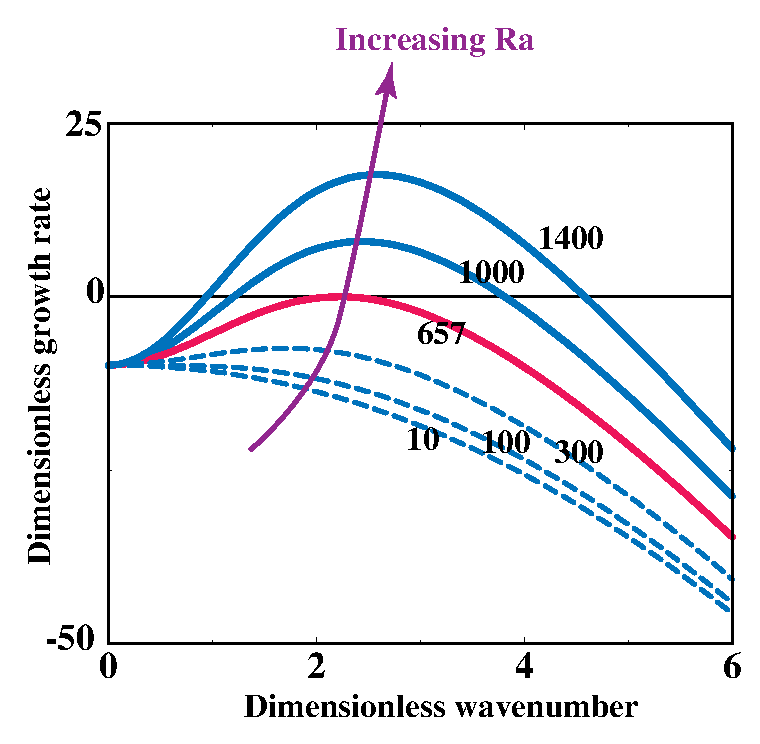
\includegraphics[width=70mm]{Diagrams/crit_ra}
				\caption[]{Critical Rayleigh Number determination. A plot of growth rates for
				harmonic perturbations as a function of wavenumber for different ${\rm Ra}$. The
				critical value occurs when the maximum of the curve just touches the horizontal
				axis at zero.}
			\end{center}	
		\end{figure}
		
		Substituting for the perturbations into the biharmonic equation and the linearized 
		energy conservation equation gives
			\begin{equation}
				\left(\frac{d^2}{d{x_2}^2} -k^2 \right)^2 \Psi = -{\rm Ra} k \Theta	
				\label{eq:psitheta1}
			\end{equation}
		and
			\begin{equation}
				\sigma \Theta + k \Psi = 	\left(\frac{d^2}{d{x_2}^2} -k^2 \right) \Theta
			\end{equation}	
			
		Here we have shown and used the fact that 
			\begin{equation}
				\nabla^2 \equiv \left(\frac{\partial^2}{\partial {x_2}^2} -k^2 \right)
				\label{eq:psitheta2}
			\end{equation}	
		when a function is expanded in the form $\phi(x,z) = \Phi(z).\sin kx$ 
		-- more generally, this is the fourier transform of the Laplacian operator.
		
		Eliminating $\Psi$ between (\ref{eq:psitheta1}) and (\ref{eq:psitheta2}) gives
			\begin{equation}
				\sigma \left(\frac{d^2}{d {x_2}^2 } - k^2 \right)^2 -{\rm Ra} k^2 \Theta = 
				\left(\frac{d^2}{d {x_2}^2} -k^2 \right)^3 \Theta
			\end{equation}
		This has a solution 
			\begin{equation}
				\Theta = \Theta_0 \sin \pi z
			\end{equation}
		which satisfies all the stated boundary conditions and implies
			\begin{equation}
				\sigma =  \frac{k^2 {\rm Ra}}{(\pi^2 + k^2)^2} -(\pi^2 + k^2)
			\end{equation}
		a real function of $k$ and $\rm Ra$.	
	
		For a given wavenumber,
		what is the lowest value of $\rm Ra$ for which perturbations at that
		wavenumber will grow ? 
			\begin{equation}
				= \frac{(\pi^2 + k^2)^3}{k^2}
			\end{equation}
		The absolute minimum value of ${\rm Ra}$ which produces growing perturbations
		is found by differentiating ${\rm Ra_0} $ with respect to $k$ and 
		setting equal to zero to find the extremum.
			\begin{equation}
				{\rm Ra_c} = \frac{27}{4} \pi^4 = 657.51
			\end{equation}
		for a wavenumber of 
			\begin{equation}
				k = \frac{\pi}{2^{1/2}} = 2.22
			\end{equation}	
		corresponding to a wavelength of 2.828 times the depth of the layer.
		
		Different boundary conditions produce different values of the critical Rayleigh number.
		If no-slip conditions are used, for example, then the $\Theta$ solution applied
		above does not satisfy the boundary conditions. In general, the critical Rayleigh
		number lies between about 100 and 3000.	
			
\subsection{Boundary layer theory, Boundary Rayleigh Number}
	
	Having determined the conditions under which convection will develop,
	we next consider what can be calculated about fully developed convection --
	i.e. when perturbations grow well beyond the linearization used
	to study the onset of instability.
	
	Let's consider fully developed convection with high Rayleigh number. From
	observations of real fluids in laboratory situations, it is well known
	how this looks. High Rayleigh number convection is dominated by the advection
	of heat. Diffusion is too slow to carry heat far into the fluid before the buoyancy
	anomaly becomes unstable. This leads to thin, horizontal ``boundary layers'' where diffusive
	heat transfer into and out of the fluid occurs. These are separated by approximately
	isothermal regions in the fluid interior. The horizontal boundary layers are connected
	by vertical boundary layers which take the form of sheets or cylindrical plumes depending
	on a number of things including the Rayleigh number. For the time being we consider
	only the sheet like downwellings since that allows us to continue working in 2D.
	
	 %% FIGURE: Simple, flat boundary layer theory
		\begin{figure}[h]
			\begin{center}
			%	\epsfxsize=10cm \epsfbox{:Diagrams:blt.eps}
				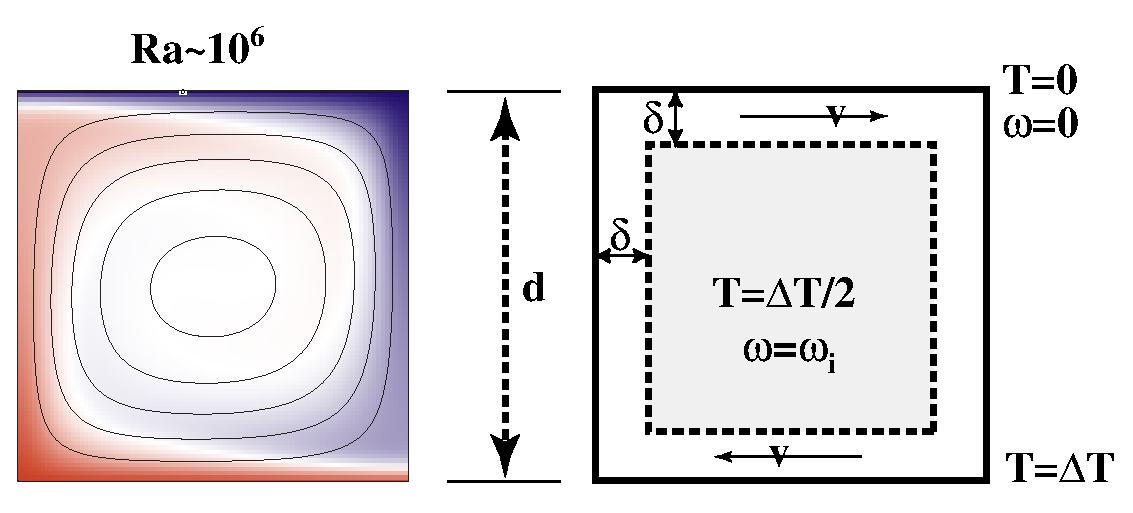
\includegraphics[width=100mm]{Diagrams/blt}
				\caption[]{ \label{fig:blt1}
					Boundary Layer Theory in its simplest form}
			\end{center}	
		\end{figure}
		
	Boundary layer analysis is a highly sophisticated field, and is used in a broad
	range of situations where differences in scales between different physical
	effects produce narrow accommodation zones where the `weaker' term
	dominates (e.g viscosity in `invicid' flow around an obstacle).
	
	Here we first make a wild stab at an approximate theory describing the
	heat flow from a layer with a given Rayleigh number. The convective
	flow is shown in Figure \ref{fig:blt1} together with our rough sketch of
	what actually happens. 
	
	Assuming the simplified flow pattern of the sketch, steady state, and replacing all derivatives
	by crude differences we obtain (using a vorticity form)
		\begin{equation}
				\kappa \nabla^2 T = (\mathbf{v} \cdot \nabla) T
					\mbox{\hspace{1cm}} \longrightarrow \mbox{\hspace{1cm}} 
				\frac{v \Delta T}{d} \sim \frac{\Delta T \kappa}{\delta^2} 
		\end{equation}
	and
		\begin{equation}
				\nabla^2 \omega = \frac{g \rho \alpha}{\eta} \frac{\partial T}{\partial x}
					\mbox{\hspace{1cm}} \longrightarrow \mbox{\hspace{1cm}} 
				\frac{\omega}{\delta ^2}	\sim  \frac{g \rho \alpha \Delta T}{\eta \delta}
		\end{equation}
	where $\omega\sim v / d$ from the local rotation interpretation of
	vorticity and the approximate rigid-body rotation of the core of the convection cell,
	and $v/d \sim \kappa / \delta^2$.
		
	This gives
		\begin{align}
			\frac{\delta}{d} & \sim {\rm Ra}^{-1/3} \\
			v & \sim \frac{\kappa}{d} {\rm Ra}^{2/3} 
		\end{align}	
	
	This theory balances diffusion of vorticity and temperature across and out of the 
	boundary layer with advection of each quantity along the boundary layer to maintain
	a steady state.
	
	The Nusselt number is the ratio of advected heat transport to that purely 
	conducted in the absence of fluid motion, or, using the above approximations,
		\begin{equation}
			\begin{split}	
				{\rm Nu} 	& \sim \frac{\rho C_p v \Delta T \delta}{(k \Delta T/d)d} \\
								& \sim {\rm Ra}^{1/3}
			\end{split}
		\end{equation}
	
	This latter result being observed in experiments to be in reasonably
	good agreement with observation. 
	
	If we define a boundary Rayleigh number
		\begin{equation}
			{\rm Ra_b} = \frac{g \rho \alpha \Delta T \delta^3}{\kappa \eta}
		\end{equation}
	then the expression for $\delta$ gives
		\begin{equation}
			{\rm Ra_b} \sim 1
		\end{equation}	
	so the boundary layer does not become more or less stable with increasing Rayleigh
	number (this is not universal -- for internal heating the boundary layer
	becomes less stable at higher Rayleigh number).	
	
	 %% FIGURE: Boundary layer plus cooling effects
		\begin{figure}[h]
			\begin{center}
				%\epsfxsize=10cm \epsfbox{:Diagrams:blt2.eps}
				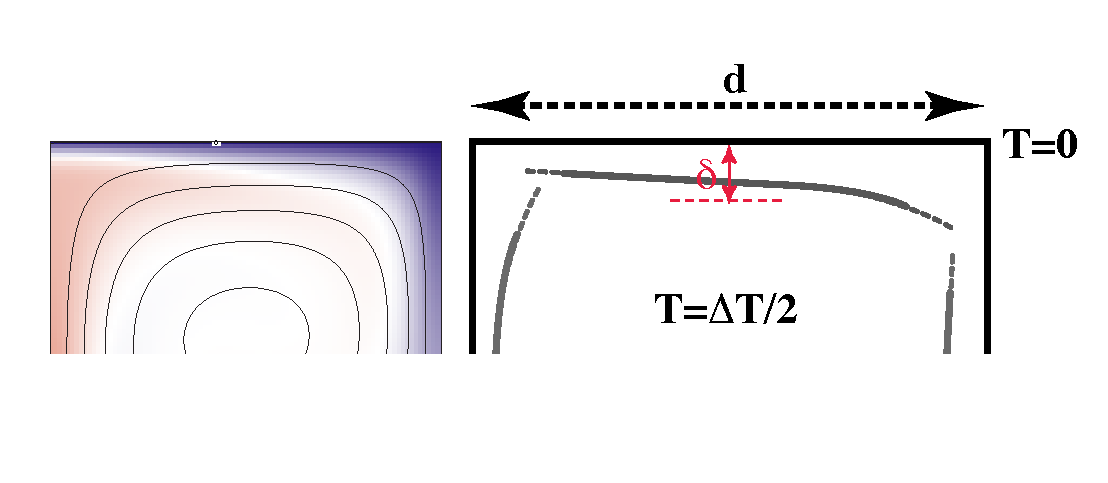
\includegraphics[width=100mm]{Diagrams/blt2}
				\caption[]{Boundary Layer Theory which accounts for the thickness variations along the 
					boundary layer as it matures.}
			\end{center}	
		\end{figure}
	
	Another wrinkle can be added to the boundary layer theory by trying to account for
	the variation  in the boundary layer thickness as it moves along the horizontal boundary.
	This refinement in the theory can account for the form of this thickness, the potential energy
	change in rising or sinking plumes, and the aspect ratio of the convection (width to height of
	convection roll) by maximizing Nusselt number as a function of aspect ratio.
	
	Consider the boundary layer to be very thin above the upwelling plume (left side). As it moves
	to the right, it cools and the depth to any particular isotherm increases (this is clearly
	seen in the simulation). This can be treated exactly like a one dimensional problem if we
	work in the Lagrangian frame of reference attached to the boundary layer. That is,
	take the 1D half-space cooling model and replace the time with $x_1/v$ (cf. the advection
	equation in which time and velocity / lengths are mixed).
	
	The standard solution is as follows. Assume a half-space at an intial
	temperature everywhere of $T_0$ to which a boundary condition, $T=T_s$ is applied
	at $t=0,x_2=0$. 
	
	 
	We solve for $T(x_2,t)$ by first making a substitution, 
			\begin{equation}	
			\theta = \frac{T-T_0}{T_s-T_0} 	
		\end{equation}
	which is a dimensionless temperature, into the standard diffusion equation to obtain	
		\begin{equation}
			\frac{\partial \theta(x_2,t)}{\partial t} = \kappa \frac{\partial ^2 \theta(x_2,t)}{\partial {x_2}^2}
			\label{eq:difftheta}
		\end{equation}	
	
	The boundary conditions on $\theta$ are simple:
	%%	\begin{equation}
			\begin{align}
				& \theta(x_2,0) = 0	\\
				& \theta(0,t) = 1	\\
				& \theta(\infty,0) = 0		
			\end{align}
	%%	\end{equation}
	%% FIGURE: Cooling half space
		\begin{figure}[h]
			\begin{center}
				%\epsfxsize=10cm \epsfbox{:Diagrams:cool.eps}
				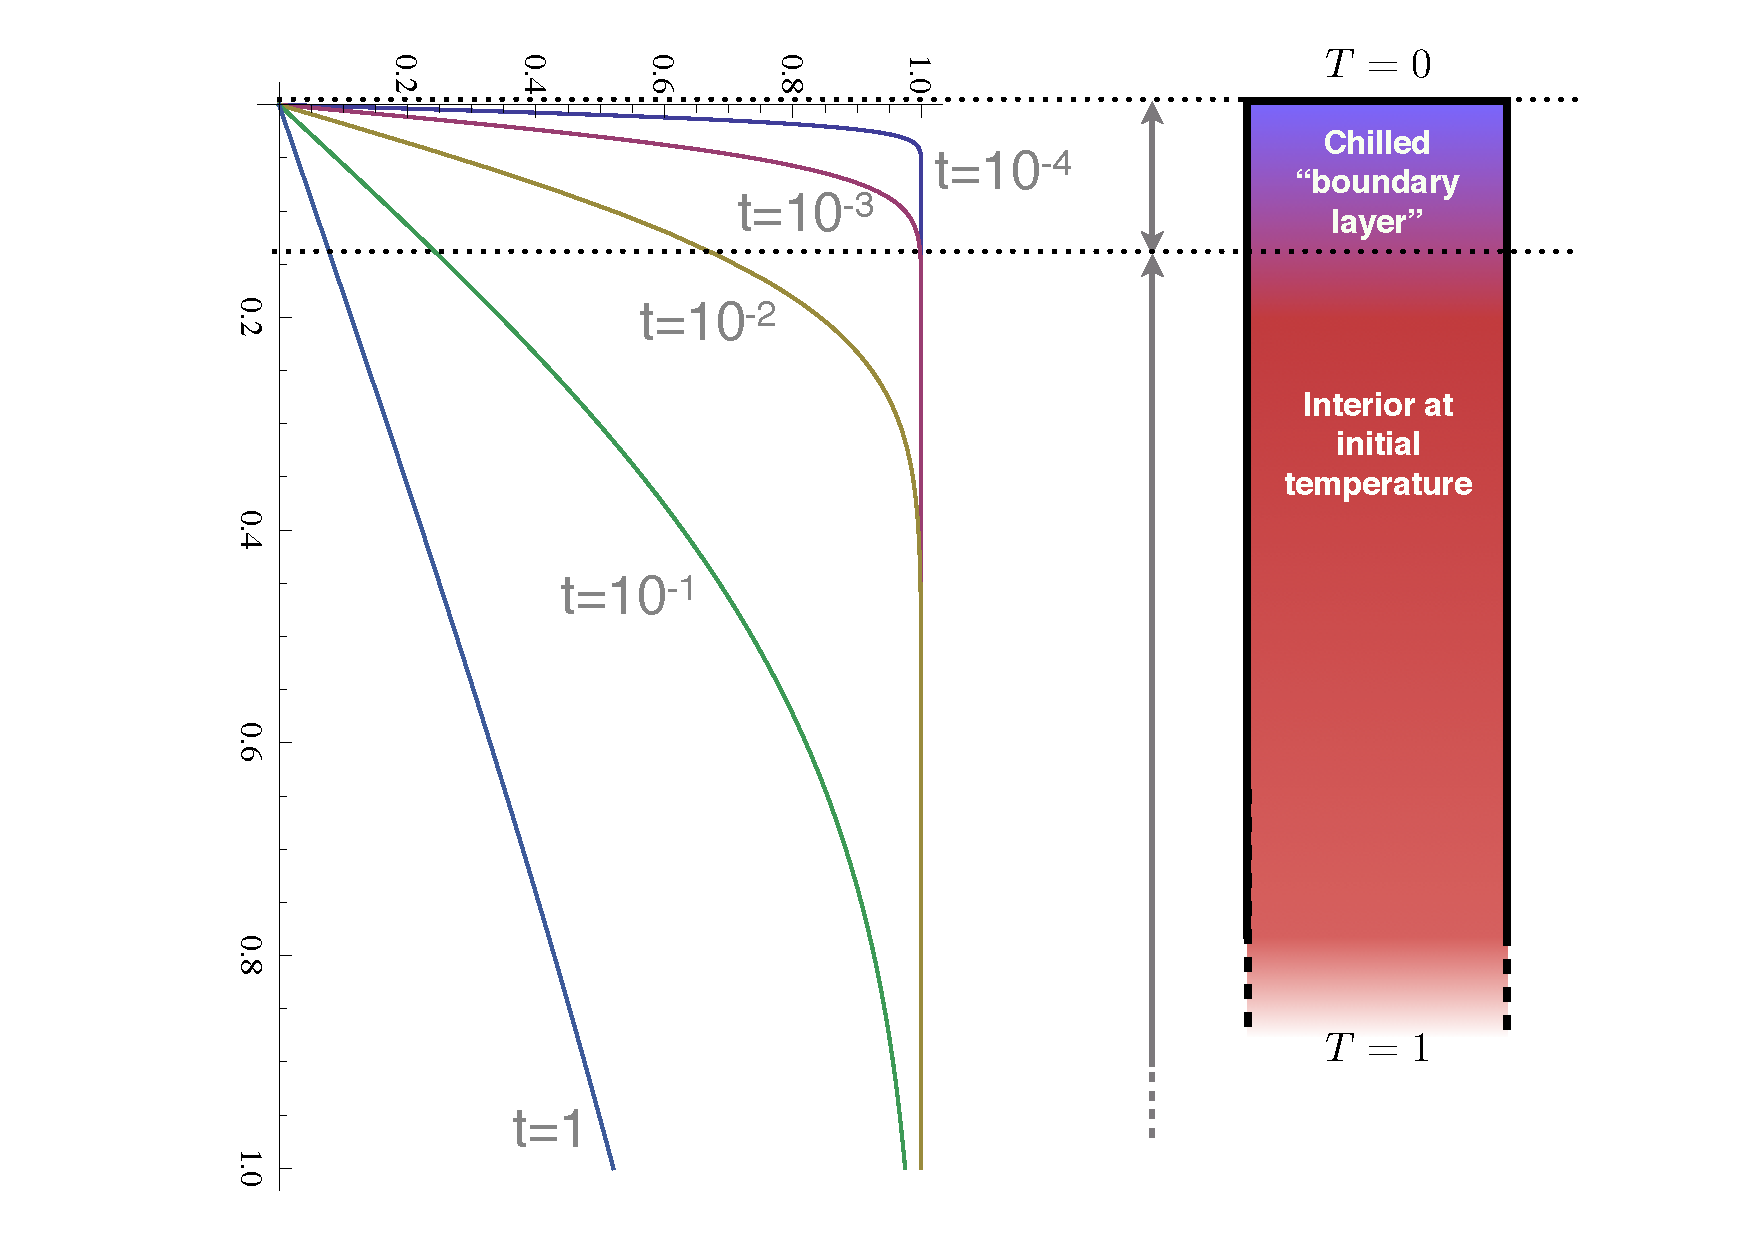
\includegraphics[width=0.66\linewidth]{Diagrams/CoolingHalfSpaceSolutions1}
				\caption[]{Cooling half-space calculation}
			\end{center}	
		\end{figure}

	In place of $t,x_2$, we use the similarity transformation,
		\begin{equation}
			\eta = \frac{x_2}{2\sqrt{\kappa t}}
		\end{equation}
	which is found (more or less) intuitively. 
	Now we need to substitute
		\begin{align}
			\frac{\partial \theta}{\partial t} & = -\frac{d \theta}{d\eta}(\eta/2t)	\\
			\frac{\partial^2 \theta}{\partial {x_2}^2} & = \frac{1}{4\kappa t}\frac{d^2 \theta}{d \eta^2}
		\end{align}
	to transform (\ref{eq:difftheta}) into
		\begin{equation}
			-\eta \frac{d \theta}{d\eta} = \frac{1}{2} \frac{d^2 \theta}{d \eta^2}
			\label{eq:diffode}
		\end{equation}
		
	Boundary conditions transform to give	
		%% \begin{equation}
			\begin{align}
				& \theta(\eta=\infty) = 0	\\
				& \theta(\eta=0) = 1	
			\end{align}
		%% \end{equation}
		
	Write $\phi = d\theta / d\eta$ (for convenience only) to rewrite (\ref{eq:diffode})
	as
		%%\begin{equation}
			\begin{align}
				-\eta \phi &= \frac{1}{2} \frac{d \phi}{d \eta}		\\
			\intertext{or}
				-\eta d\eta &= \frac{1}{2} \frac{d\phi}{\phi}	
			\end{align}	
		%%\end{equation}
	
	This is a standard integral with solution
		%%	\begin{equation}
			\begin{align}
				& -\eta^2 = \log_e \phi -\log_e c_1 \\
			\intertext{such that}
				& \phi = c_1 \exp(-\eta^2) = \frac{d\theta}{d\eta}
			\end{align}	
		%% \end{equation}
		
	This latter form is then integrated to give the solution:
		\begin{equation}
			\theta = c_1 \int_0^\eta 	\exp(-{\eta'}^2) d\eta' +1
		\end{equation}	
	Boundary conditions give	
		\begin{equation}
			\theta = 1- \frac{2}{\sqrt{\pi}} \int_0^\eta\exp(-{\eta'}^2) d\eta'
		\end{equation}	
		
	Which is the definition of the complementary error function ($\erfc(\eta)$).	
			
	Undoing the remaining substitutions gives
		\begin{equation}
				\frac{T-T_0}{T_s-T_0} 	= \erfc \left(   \frac{x_2}{2\sqrt{\kappa t}} \right)
		\end{equation}
		
	In our original context of the cooling boundary layer, then, the $T_	s$ is the surface
	temperature, $T_0$ is the interior temperature of the convection cell ($\Delta T /2$)
	and $t \leftarrow x_1/v$. The thickness of the boundary layer is found by assuming
	it is defined by a characteristic isotherm (doesn't much matter which). The
	progression of this isotherm is 
		\begin{equation}
			\delta \propto \sqrt{\kappa t}  
		\end{equation}
	or, in the Eulerian frame 
		\begin{equation}
			\delta \propto \sqrt{\kappa x_1 / v}  
		\end{equation}	
			
	\subsection{Internal Heating}	
	
	The definition of the Rayleigh number when the layer is significantly
	internally heated is
		\begin{equation}
			{\rm Ra} = \frac{g \rho^2 \alpha H d^5}{\eta \kappa k}
		\end{equation}
	where $H$ is the rate of internal heat generation per unit mass.
	
	The rigorous definition of the Nusselt number is the heat flow 
	through the upper surface divided by the average basal temperature. This
	allows a Nusselt number to be calculated for internally heated convection
	where the basal temperature is not known {\em a priori}
	
	Internally heated convection is a problem to simulate in the lab, directly, but
	the same effect is achieved by reducing the temperature of the upper surface as a function of
	time.
	
	\subsection{When Viscosity is Not Constant}
	
		When viscosity is not constant, the equations are considerably complicated.
		It is no longer possible to form a pure biharmonic equation since $\eta(x,z)$ cannot
		be taken outside the differential operators. Nor can stream-function / vorticity formulations
		be used directly for the same reasons. Spectral methods — the decomposition 
		of the problem into a sum of independent problems in the wavenumber domain —
		is no longer simple since the individual problems are coupled, not independent.
		
		The Rayleigh number is no longer uniquely defined for the system since
		the viscosity to which it refers must take some suitable average over the 
		layer — the nature of this average depends on the circumstances.
		
		The form of convection changes since boundary layers at the top and
		bottom of the system (cold v hot) are no longer symmetric with each other.
		
		The convecting system gains another control parameter which is a measure of the
		viscosity contrast as a function of temperature.
	
\section{Application to Planets}
	
		%% Discussion topic !!
	
		The application of realistic convection models to the
		Earth and other planets — particularly Venus.
		
		The simplest computational and boundary layer solutions to the Stokes' convection
		equations made the simplifying assumption that the viscosity 
		was constant. Despite the experimental evidence which suggests viscosity 
		variations should dominate in the Earth, agreement with some 
		important observations was remarkably good.

		The simulations were not able to produce plate-like motions
		at the surface (instead producing smoothly distributed deformation) but
		the average velocity, the heat flow and the observed pattern of subsidence
		of the ocean floor were well matched.
		
		\subsection{Mantle Rheology}
		
			Experimental determination of the rheology of mantle materials
			gives 
				\begin{equation}
					\dot{\epsilon} \propto \sigma^n d^{-m} \exp\left( -\frac{E+PV}{RT} \right)
				\end{equation}
			where $\sigma$ is a stress, $d$ is grain size, $E$ is an activation energy, $V$ is
			an activation volume, and $T$ is absolute temperature. ($R$ is the universal gas
			constant).
			
			This translates to a viscosity
				\begin{equation}
					\eta \propto \sigma^{1-n} d^m exp\left( \frac{E+PV}{RT} \right)
				\end{equation}
		
			In the mantle two forms of creep are possible, dislocation creep with $n ~ 3.0$, $m~0$,
			$E ~ 430-540 KJ/mol$, $V ~ 10 - 20 cm^3/mol$; and diffusion creep with $n ~ 1.0$, $m~2.5$,
			$E ~ 240-300 KJ/mol$, $V ~ 5-6 cm^3/mol$. This is for olivine --- other minerals will 
			produce different results, of course.
			
		
		\subsection{Convection with Temperature Dependent Viscosity}

		More sophisticated models included the effect of temperature dependent 
		viscosity as a step towards more realistic simulations. In fact, the opposite was observed: 
		convection with temperature dependent viscosity is a much worse description of the 
		oceanic lithosphere than constant viscosity convection. It may, however, 
		describe Venus rather well.

		Theoretical studies of the asymptotic limit of convection in which the viscosity variation 
		becomes very large (comparable to values determined for mantle rocks in 
		laboratory experiments) find that the upper surface becomes entirely stagnant with 
		little or no observable motion. Vigorous convection continues underneath the stagnant layer
		with very little surface manifestation. 

		This theoretical work demonstrates that the 
		numerical simulations are producing correct results, and suggests that we should look
		for physics beyond pure viscous flow in explaining plate motions.
		
		
	\subsection{Non-linear Viscosity and Brittle Effects}	
	
		Realistic rheological laws show the viscosity may depend
		upon stress. This makes the problem non-linear since the
		stress clearly depends upon viscosity.
		In order to obtain a solution it is necessary to iterate
		velocity and viscosity until they no longer change.
		
		The obvious association of plate boundaries with earthquake activity suggests 
	that relevant effects are to be found in the brittle nature of the cold plates. Brittle
	materials have a finite strength and if they are stressed beyond that point they break. This
	is a familiar enough property of everyday materials, but rocks in the lithosphere are non-uniform, 
	subject to great confining pressures and high temperatures, and they deform over extremely long
	periods of time. This makes it difficult to know how to apply laboratory results for rock
	breakage experiments to simulations of the plates.

	An ideal, very general rheological model for the brittle lithosphere would incorporate the effects
	due to small-scale cracks, faults, ductile shear localization due to dynamic recrystalization, 
	anisotropy (... kitchen sink). Needless to say, most attempts to date to account for the
	brittle nature of the plates have greatly simplified the picture. Some models have imposed weak
	zones which represent plate boundaries, others have included sharp discontinuities which represent
	the plate-bounding faults, still others have used continuum methods in which the yield properties
	of the lithosphere are known but not the geometry of any breaks.
	Of these approaches, the continuum approach is best able to demonstrate the spectrum of
	behaviours as convection in the mantle interacts with brittle lithospheric plates. For studying
	the evolution of individual plate boundaries  methods which explicitly include 
	discontinuities work best.
	
	The simplest possible continuum formulation includes a yield stress expressed 
	as an non-linear effective viscosity.
			\begin{equation}
				\eta_{\rm eff} = \frac{\tau_{\rm yield}}{\dot{\varepsilon}}
			\end{equation}
	This formulation can be incorporated very easily into the mantle dynamics modeling approach
	that we have outlined above as it involves making modifications only to the viscosity law.
	There may be some numerical difficulties, however, as the strongly non-linear rheology can
	lead to dramatic variations in the viscosity across relatively narrow zones.
	
	
%TODO: Plasticity more generally

%TODO: Figure for non-linear rheology	
	
	
	
	
	
		
	\section{Thermochemical Convection}
	
		The Rayleigh number is defined in terms of thermal
		buoyancy but other sources of buoyancy are possible in fluids.
		
		For example, in the oceans, dissolved salt makes water heavy. When
		hot salty water (e.g. the outflows of shallow seas such as the Mediterranean)
		mixes with cold less salty water, there is a complicated interaction.
		
		This is double diffusive convection and produces 
		remarkable layerings etc since the diffusion coefficients 
		of salt and heat are different by a factor of 100.
		
		In the mantle, bulk chemical differences due to subduction of 
		crustal material can be treated in a similar manner. From the point
		of view of the diffusion equations, the diffusivity of bulk chemistry in
		the mantle is tiny (pure advection).
		
		Fluid flows with chemical v. thermal bouyancy are termed
		thermochemical convection problems. 
		
	
	\section{Other Applications and Analytic Results}
	
	\subsection{Rayleigh-Taylor Instability \& Diapirism}
		%% FIGURE: sketch of salt diapir formation
		\begin{figure}[h]
			\begin{center}
			%	\epsfxsize=10cm \epsfbox{:Diagrams:diapirs.eps}
				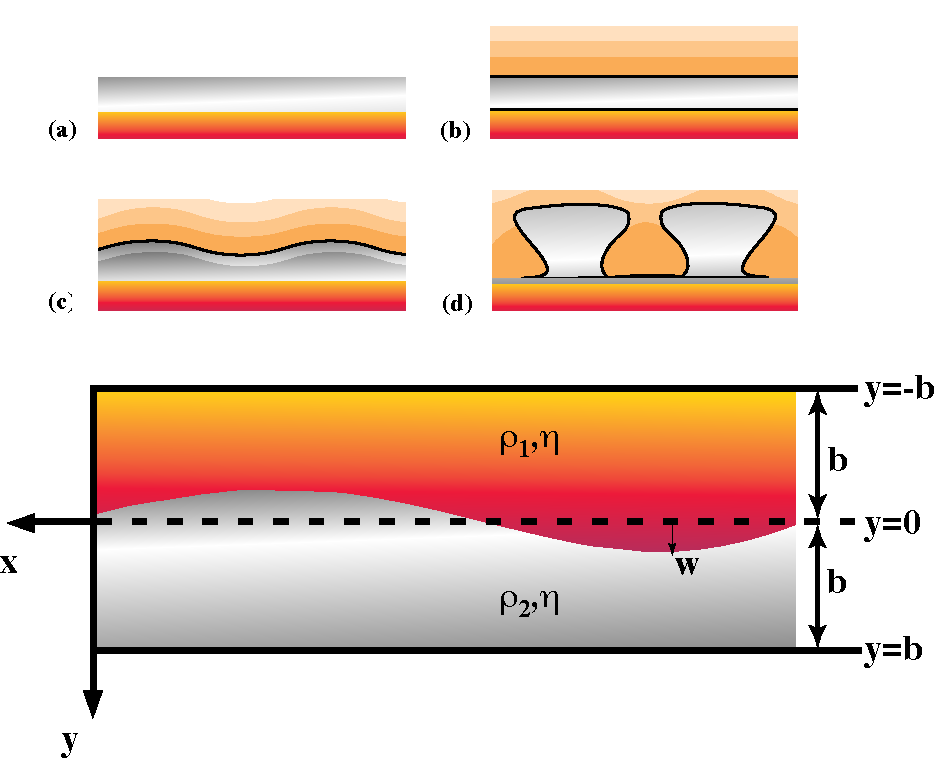
\includegraphics[width=100mm]{Diagrams/diapirs}
				\caption[]{
					Salt diapirs result when a buried layer of salt(a,b) becomes
					convectively unstable and rises through the overlying sediment layers (c,d).
					The idealized geometry for the Rayleigh-Taylor instability problem
					is outlined in the lower diagram}
				\label{fig:raytay}
			\end{center}	
		\end{figure}
		
	Diapirism is the buoyant upwelling of rock which is lighter
	than its surroundings. This can include mantle plumes and 
	other purely thermal phenomena but it often applied to 
	compositionally distinct rock masses such as melts infiltrating
	the crust (in the Archean) or salt rising through denser sediments.
	
	Salt layers may result from the evaporation of seawater. If subsequent
	sedimentation covers the salt, a gravitionally unstable configuration results with
	heavier material (sediments) on top of light material (salt). The rheology
	of salt is distinctly non-linear and also sensitive to temperature. Once buried, the 
	increased temperature of the salt layer causes its viscosity to decrease to the 
	point where instabilities can grow. Note, since there is always a strong density 
	contrast between the two rock types, the critical Rayleigh number argument
	does not apply -- this situation is always unstable, but instabilities can only
	grow at a reasonable rate once the salt has become weak.
	
	The geometry is outlined above in Figure ({\ref{fig:raytay}). We suppose
	initially that the surface is slightly perturbed with a form of
		\begin{equation}
			w_m = w_{m0} \cos kx
		\end{equation}
		
	where $k$ is the wavenumber, $k=2\pi / \lambda$, $\lambda$ being the wavelength
	of the disturbance. We assume that the magnitude of the disturbance is always
	much smaller than the wavelength. 
	
	The problem is easiest to solve if we deal with the biharmonic equation
	for the stream function. Experience leads us to try to separate 
	variables and look for solutions of the form
		\begin{equation}
			\psi = \left( A \sin kx + B \cos kx \right ) Y(y) 
		\end{equation}
	
	where the function $Y$ is to be determined. The form we have chosen
	for $w_m$ in fact means $A=1,B=0$ which we can assume from now on to
	simplify the algebra.
	
	Substituting the trial solution for $\psi$ into the biharmonic
	equation gives
		\begin{equation}
			\frac{d^4 Y}{d y^4} -2k^2 \frac{d^2 Y}{dy^2} +k^4 Y = 0
		\end{equation} 
	 
	 which has solutions of the form 
	 	\begin{equation}
	 		Y = A \exp(m y)
	 	\end{equation}
	where $A$ is an arbitrary constant.	Subtituting gives us an equation for $m$	
		\begin{equation}
			m^4 - 2 k^2 m^2 + k^4 = (m^2 - k^2)^2 = 0
			\label{eq:diapaux}
		\end{equation}
	or
		\begin{equation}
			m = \pm k
		\end{equation}

	Because we have degenerate eigenvalues (i.e. of the four
	possible solutions to the auxilliary equation (\ref{eq:diapaux}),
	two pairs are equal) we need to extend the form of the solution 
	to 
		\begin{equation}
			Y = (By+A) \exp(m y)
		\end{equation}	
	to give the general form of the solution in this 
	situation to be
		\begin{align}
			\psi &= \sin kx \left( A e^{-ky} + B y e^{-ky} + C e^{ky} + D y e^{ky} \right)
			\label{eq:biharmsoln1} \\
		\intertext{or, equivalently}
			\psi &= \sin kx \left( A_1 \cosh ky + B_1 \sinh ky + C_1 y \cosh ky + D_1 y \sinh ky  \right)
			\label{eq:biharmsoln2} 
		\end{align}	
	
	This equation applies in each of the layers separately. We therefore need to find
	two sets of constants $\{A_1,B_1,C_1,D_1\}$ and $\{A_2,B_2,C_3,D_4\}$ by the
	application of suitable boundary conditions. These are known in terms of the
	velocities in each layer, $\mathbf{v}_1 = \mathbf{i} u_1 +\mathbf{j} v_1$ and
	$\mathbf{v}_2 = \mathbf{i} u_2 +\mathbf{j} v_2$:
		%% \begin{equation}
			\begin{align}
				u_1 = v_1 &= 0 \text{\hspace{1cm} on \hspace{1cm}} y = -b \\
				u_2 = v_2 &= 0 \text{\hspace{1cm} on \hspace{1cm}} y = b 
			\end{align}
		%% \end{equation}
		
	together with a continuity condition across the interface (which we 
	assume is imperceptibly deformed} 	
		\begin{equation}
				u_1 = u_2  \text{\hspace{1cm} and \hspace{1cm}} 
				v_1 = v_2 \text{\hspace{1cm} on \hspace{1cm}} y = 0 
		\end{equation}
	
	The shear stress ($\sigma_{xy}$) should also be continuous across the interface,
	which, if we assume equal viscosities, gives
		\begin{equation}
			\frac{\partial u_1}{\partial y} + \frac{\partial v_1}{\partial x} =
			\frac{\partial u_2}{\partial y} + \frac{\partial v_2}{\partial x} \text{\hspace{1cm} on \hspace{1cm}} y = 0 
		\end{equation}
	and, to simplify matters, if the velocity is continuous across $y=0$ then any 
	velocity derivatives in the $x$ direction evaluated at $y=0$ will also be
	continuous (i.e. $\partial v_2 / \partial x = \partial v_1 / \partial x$).
		
	The expressions for velocity in terms of the solution (\ref{eq:biharmsoln2}) are
		\begin{subequations}
			\begin{align}
				u  = -\frac{\partial \psi}{\partial y} & = -\sin kx \left( 
								(A_1 k + D_1 + C_1 k y) \sinh ky + (B_1 k + C_1 + D_1 ky) \cosh ky	\right) \\
				v  = \frac{\partial \psi}{\partial x} & = k \cos kx \left( 
								(A_1 +C_1 y)\cosh ky + (B_1 +D_1 y)  \sinh ky 	\right)
			\end{align}
		\end{subequations}	
		
	From here to the solution requires much tedious rearrangement, and the usual argument
	based on the arbitrary choice of wavenumber $k$ but we finally arrive at	
		\begin{multline}
			\psi_1 = A_1 \sin kx \cosh ky + \\
							A_1 \sin kx \left[ 	
								\frac{y}{k b^2} \tanh kb \sinh ky + 
										\left( \frac{y}{b} \cosh ky    \frac{1}{kb} \sinh ky \right) \cdot 
										\left( \frac{1}{kb} + 
										\frac{1}{\sinh bk \cosh bk} \right) \right] \times \\
							\left[ \frac{1}{\sinh bk \cosh bk} - \frac{1}{(b^2k^2} \tanh bk \right] ^{-1} 	
			\label{eq:raytays1}				
		\end{multline}	
	The stream function for the lower layer is found by replacing $y$ with $-y$ in this 
	equation.	 This is already a relatively nasty expression, but we haven't finished since
	the constant $A_1$ remains. This occurs because we have so far considered the form
	of flows which satisfy all the boundary conditions but have not yet considered
	what drives the flow in each layer.
	
	To eliminate $A_1$, we have to consider the physical scales inherent in the 
	problem itself. We are interested (primarily) in the behaviour of the interface
	which moves with a velocity $\partial w / \partial t$. As we are working with
	small deflections of the interface, 
		\begin{equation}
			\frac{\partial w}{\partial t} = \left. v \right|_{y=0}
		\end{equation}
	
		%% FIGURE: sketch of salt diapir formation
		\begin{figure}[h]
			\begin{center}
				%\epsfxsize=10cm \epsfbox{:Diagrams:diapir2.eps}
				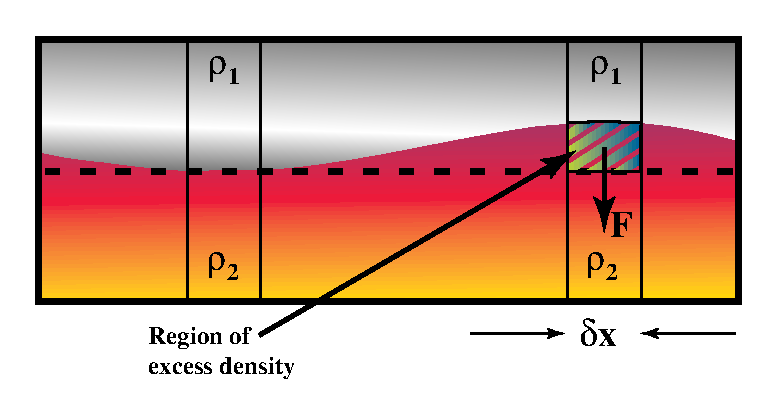
\includegraphics[width=100mm]{Diagrams/diapir2}
				\caption[]{
					The restoring force for a stable layering is proportional to
					the excess density when a fluid element is displaced across
					the boundary}
				\label{fig:raytay2}
			\end{center}	
		\end{figure}
	
	Consider what happens when the fluid above the interface is lighter than
	the fluid below -- this situation is stable so we expect the layering to 
	be preserved, and if the interface is disturbed the disturbance to decay.
	This implies that there must be a restoring force acting on  an element
	of fluid which is somehow displaced
	across the boundary at $y=0$ (Figure \ref{fig:raytay2}).   
	
	This restoring force is due to the density difference between the displaced
	material and the layer in which it finds itself. The expression for the force
	is exactly that from Archimedes principle which explains how a boat can 
	float (only in the opposite direction)
		\begin{equation}
			\left. F_2 \right|_{y=0} = \delta x g w (\rho_2 - \rho_1) 
		\end{equation}
	which can be expressed as a normal stress difference (assumed to apply, once again,
	at the boundary). The viscous component of the normal stress turns out to be zero --
	proven by evaluating $\partial v / \partial y$ at $y=0$ using the expression for
	$\phi$ in equation (\ref{eq:raytays1}). Thus the restoring stress is purely pressure
		\begin{equation}	
			\left. P_2 \right|_{y=0} = g w (\rho_2 - \rho_1)
		\end{equation}
		
	The pressure in terms of the solution (so far) for $\psi$ is found
	from the equation of motion in the horizontal direction 
	(substituting the stream function formulation) 
	and is then equated to the restoring pressure above.
		\begin{equation}
			(\rho_1-\rho_2) g w = -\frac{4 \eta k A_1}{b} \cos kx 
					\left(\frac{1}{kb} + \frac{1}{\sinh bk \cosh bk} \right) \cdot
					\left(   \frac{1}{\sinh bk \cosh bk} - \frac{1}{(b^2k^2} \tanh bk \right)^{-1}												
		\end{equation}
	which allows us to substitute for $A_1$	in our expression for $\partial w / \partial t$
	above. Since $A_1$ is independent of $t$, we can 
	see that the solution for $w$ will be of a growing or 
	decaying exponential form with growth/decay constant
	coming from the argument above.
		\begin{equation}
			w(t) = w_0 \exp((t-t_0)/\tau)	
		\end{equation}
	where
		\begin{equation}
			\tau = \frac{4 \eta}{(\rho_1-\rho_2) g b} \left( \frac{1}{kb} + \frac{1}{\sinh bk \cosh bk} \right) \cdot
						\left(   \frac{1}{k^2b^2} \tanh kb - \frac{1}{\sinh kb \cosh kb}     \right)^{-1}
		\end{equation}
	
	So, finally, an answer -- the rate at which instabilities on the interface between two
	layers will grow (or shrink) which depends on viscosity, layer depth and density differences, 
	together with the geometrical consideration of the layer thicknesses.  

	A stable layering results from light fluid resting on heavy fluid; a heavy fluid
	resting on a light fluid is always unstable (no critical Rayleigh number applies)
	although the growth rate can be so small that no deformation occurs in practice.
	The growth rate is also dependent on wavenumber. There is a minimum in the 
	growth time as a function of dimensional wavenumber which occurs at $k b = 2.4$, so
	instabilities close to this wavenumber are expected to grow first and dominate.
	
	Remember that this
	derivation is simplified for fluids of equal viscosity, and layers of identical depth. 
	Remember also that the solution is for {\rm infinitessimal} deformations of the 
	interface. If the deformation grows then the approximations of small deformation
	no longer hold. This gives a clue as to how difficulties dealing with the advection
	term of the transport equations arise.
	
	At some point it becomes impossible to obtain meaningful results without 
	computer simulation. However, plenty of
	further work has already been done on this area for non-linear fluids, temperature dependent viscosity
	\&c and the solutions are predictably long and tedious to read, much less solve. When the viscosity
	is not constant, the use of a stream function notation is not particularly helpful as the biharmonic
	form no longer appears.

	\Emerald{(e.g. read work by Ribe, Houseman et al.)}
	
	The methodology used here is instructive, as it can be used in a number of different applications
	to related areas. The equations are similar, the boundary conditions different.
		
	\subsubsection{Post-Glacial Rebound}	
	
	%% FIGURE: sketch of post-glacial rebound problem
		\begin{figure}[h]
			\begin{center}
				%\epsfxsize=8cm \epsfbox{:Diagrams:postglac.eps}
				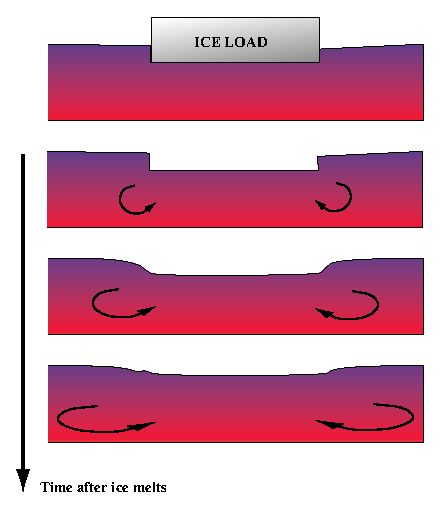
\includegraphics[width=80mm]{Diagrams/postglac}
				\caption[]{The relaxation of the Earth's surface
				after removal of an ice load.
				}
				\label{fig:postg1}
			\end{center}	
		\end{figure}
	
	In the postglacial rebound problem, consider a viscous half
	space with an imposed topography at $t=0$. The ice load
	is removed at $t=0$ and the interface relaxes back to 
	its original flat state. 
	
	This can be studied one wavenumber at a time --- computing a
	decay rate for each component of the topography. The intial
	loading is computed from the fourier transform of the 
	ice bottom topography.
	
	The system is similar to that of the diapirs except that the 
	loading is now applied to one surface rather than
	the interface between two fluids.
		
	\subsubsection{Phase Changes in the mantle}
	
	A different interface problem is that of mantle phase changes. 
	Here a bouyancy anomaly results if the phase change boundary is
	distorted. This can result from advection normal
	to the boundary bringing cooler or warmer material across
	the boundary.
	
	The buoyancy balance argument used above can be recycled
	here to determine a scaling for the ability of plumes/downwellings
	to cross the phase boundary.
	
	\subsubsection{Kernels for Surface Observables}	

	The solution method used for the Rayleigh Taylor problem 
	can also be used in determining spectral Green's functions
	for mantle flow in response to thermal perturbations. This is
	a particularly abstract application of the identical theory. 
	
	\subsection{Folding of Layered (Viscous) Medium}
	
	%% FIGURE: sketch of Biot viscous fold geometry
		\begin{figure}[h]
			\begin{center}
				%\epsfxsize=10cm \epsfbox{:Diagrams:fold.eps}
				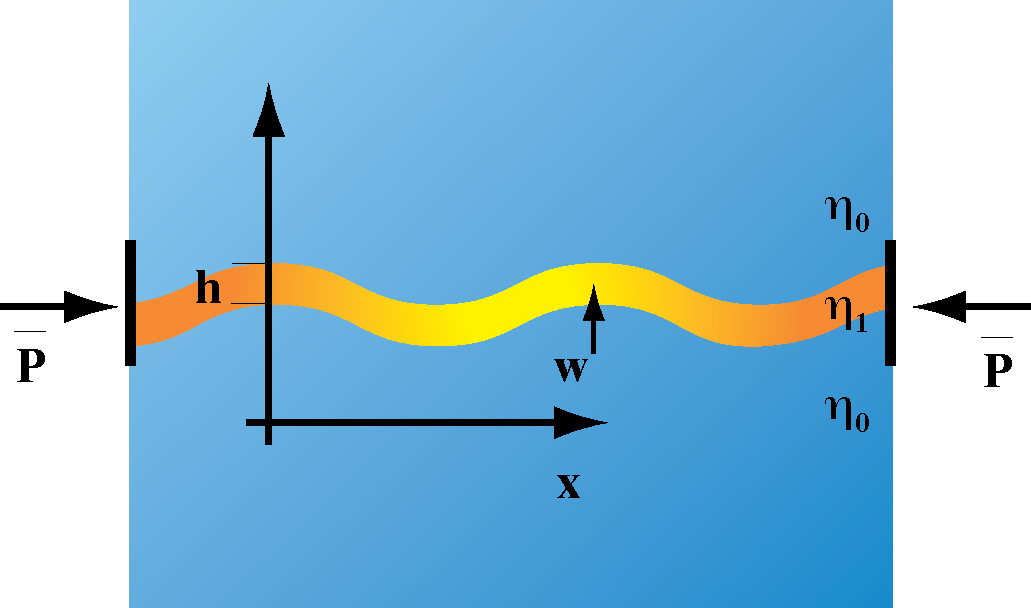
\includegraphics[width=100mm]{Diagrams/fold}
				\caption[]{Instability in a thin, viscous layer compressed
				from both ends.
				}
				\label{fig:fold1}
			\end{center}	
		\end{figure}

	
	If a thin viscous layer is compressed from one
	end then it may develop buckling instabilities 
	in which velocities grow perpendicular to the plane of
	the layer. 
	
	If the layer is
	embedded between two semi-infinite layers
	of viscous fluid with viscosity much smaller
	than the viscosity of the layer, then Biot
	theory tells us the wavelength of the initial 
	buckling instability, and the rate at which 
	it grows.
	
	The fold geometry evolves as
		\begin{equation}
			w=w_m \cos(kx) e^{\frac{t}{\tau_a}}
		\end{equation}
	where
		\begin{equation}
			\tau_a = \frac{1}{\bar{P}}\left[ \frac{4 \eta_0}{k} + \frac{\eta_1 h^3}{3k^2} \right]
		\end{equation}
	and the fastest growing wavenumber is
		\begin{equation}
			k = \frac{6}{h}\left( \frac{\eta_1}{\eta_0} \right)^{\frac{1}{3}}
		\end{equation}
	
	For large deformations we eventually must
	resort to numerical simulation.

	\subsection{Gravity Currents}
	
	%% FIGURE: sketch of gravity current evolution
		\begin{figure}[h]
			\begin{center}
				%\epsfxsize=10cm \epsfbox{:Diagrams:gravcurr.eps}
				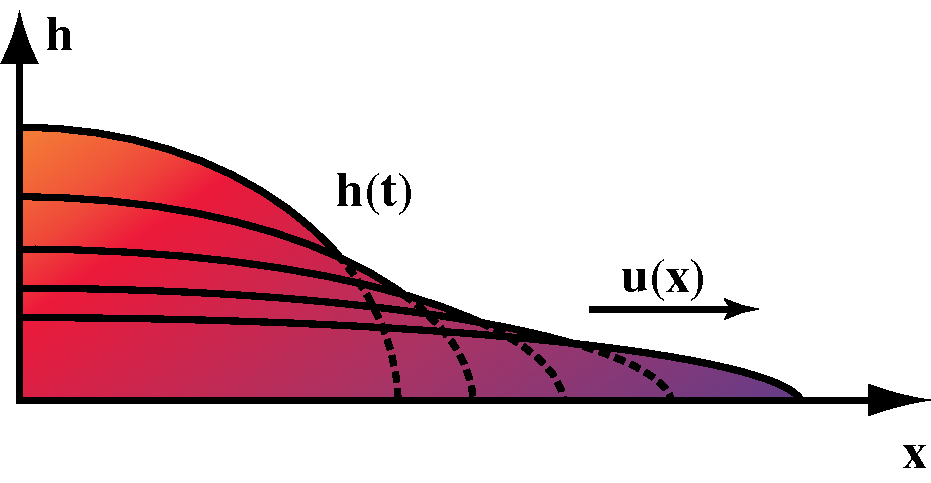
\includegraphics[width=100mm]{Diagrams/gravcurr}
				\caption[]{A gravity current is the spreading of a dense
				fluid under its own weight across a horizontal surface (or
				a buoyant fluid under a surface). Open the fridge door and
				the cold air falls out as a gravity current.
				}
				\label{fig:gcurr1}
			\end{center}	
		\end{figure}
		
		Gravity currents can occur when a viscous fluid flows under its own weight
		as shown in Figure \ref{fig:gcurr1}. 
		
		We assume that the fluid has constant viscosity, $\eta$ and that
		the length of the current is considerably greater than its height. The fluid is embedded
		in a low viscosity medium of density $\rho-\Delta \rho$ where $\rho$ is the density
		of the fluid itself.
	
		The force
		balance is between buoyancy and viscosity. The assumptions of geometry allow us
		to simplify the Stokes equation by assuming horizontal pressure gradients due to the 
		surface slope drive the flow.
			\begin{equation}
				\nabla p = \eta\nabla^2 u \approx   g \Delta \rho \frac{\partial h}{\partial x}  
			\end{equation}
		
		We assume near-zero shear stress at the top of the current to give
			\begin{equation}
				\frac{\partial u}{\partial z} (x,h,t) = 0
			\end{equation}
		and zero velocity at the base of the current.
		Hence	
			\begin{equation}
				u(x,z,t) = -\frac{1}{2} \frac{g \Delta \rho}{\eta} \frac{\partial h}{\partial x}  z(2h-z)
			\end{equation}
		
		Continuity integrated over depth implies
			\begin{equation}
				\frac{\partial h}{\partial t} + \frac{\partial }{\partial x} \int_0^h u dz = 0
			\end{equation}
		Combining these equations gives
			\begin{equation}
				\frac{\partial h}{\partial t} -\frac{1}{3} \frac{g \Delta \rho}{\eta} 
				     \frac{\partial }{\partial x}  \left( h^3 \frac{\partial h}{\partial x} \right) = 0 
			\end{equation}
	   Finally, a global constraint fixes the total amount of fluid at any given time
		   	\begin{equation}
		   		\int_0^{x_N(t)} h(x,t)dx = qt^\alpha
		   	\end{equation}		
	 The latter term being a fluid source at the origin, and $x_{N(t)}$ the 
	 location of the front of the current.
	 A similarity variable is available
	 	\begin{equation}
	 		\nu = \left( \frac{1}{3} g\Delta \rho q^3 / \eta \right)^{-\frac{1}{5}} x t^{-(3\alpha +1) / 5}
	 	\end{equation}
	giving a solution of the form
		\begin{equation}
			h(x,t) = \nu_N^{2/3} (3q^2 \eta / (g\Delta\rho))^{1/5} t^{(2\alpha -1) / 5} \phi(\nu/\nu_N)
		\end{equation}
	where $\nu_N$ is the value of $\nu$ at $x=x_N(t)$. Substituting into the equation
	for $\partial h / \partial t$ we find that $\phi(\nu/\nu_N)$ satisfies
		\begin{equation}
			\phi({\nu}/{\nu_N}) = \left[ \frac{3}{5}(3\alpha+1)\right]^{\frac{1}{3}}
				\left(1-\frac{\nu}{\nu_N} \right)^{\frac{1}{3}} \left[
				1 - \frac{3\alpha-4}{24(3\alpha+1)}\left(1-\frac{\nu}{\nu_N} \right) + O \left(1-\frac{\nu}{\nu_N} \right)^2
				\right]
		\end{equation}
	Which has an analytic solution if $\alpha=0$ (only constant sources or sinks)
		\begin{equation}
			\begin{split} 
			\phi({\nu}/{\nu_N}) &= \left( \frac{3}{10}\right)^{\frac{1}{3}} 
			\left( 1-\left(\frac{\nu}{\nu_N}\right)^2 \right)^{\frac{1}{3}}  \\						
		\nu_N &= \left[ \frac{1}{5} \left( \frac{3}{10}\right)^{\frac{1}{3}}  \pi^{\frac{1}{2}}
	\Gamma (1/3) / \Gamma (5/6) \right]^{-\frac{3}{5}} = 1.411
			\end{split}
		\end{equation}
	For all other values of $\alpha$ numerical integration schemes must be 
	used for $\phi$.

	It is also possible to obtain solutions if axisymmetric geometry is used.
	
	
\section{Reading Material} 

G.~F. Davies.
\newblock \emph{Dynamic Earth}.
\newblock Cambridge University Press, New York, 1999.

J.~Grotzinger, T.~H. Jordan, F.~Press, and R.~Siever.
\newblock \emph{{Understanding Earth}}.
\newblock W. H. Freeman \& Co, 5 edition, 2006.
\newblock URL \url{http://bcs.whfreeman.com/understandingearth5e/}.

L.~D. Landau and E.~M. Lifshitz.
\newblock \emph{Fluid Mechanics}, volume~6 of \emph{Course of Theoretical
  Physics}.
\newblock Pergamon Press, 1959.

G.~Schubert, D.~L. Turcotte, and P.~Olson.
\newblock \emph{Mantle Convection in {E}arth and Planets}.
\newblock Cambridge University Press, UK, 2001.

D.L. Turcotte and G.~Schubert.
\newblock \emph{Geodynamics}.
\newblock John Wiley and Sons, New York, 1982.

	
	
	
	
\end{document}
